%% Chapter 7 — 서빙 시스템 입문
\setcounter{chapter}{6}
\chapter{서빙 시스템 입문}
\chaptersubtitle{파트 2의 시작 — 온라인, 배치, 스트리밍, 그리고 빠름의 언어: 꼬리, 약속, 대기열, 형식}

\begin{calloutbox}{tbbblue}{tbbbluefill}
{\normalsize\bfseries\color{tbbblue}학습 목표}\par\vspace{3pt}
\begin{tbbitemize}
  \item 팀 채팅의 논쟁 하나를 바탕으로, SLO가 없는 서비스에서는 모든 불만이 장애가 되고 조용한 날은 모두 우연이 되는 이유와 "평균은 182 ms"라는 말이 실제로는 아무도 설명하지 못하는 이유를 진단한다.
  \item "누가 무엇을 기다리는가?"를 물어 워크로드를 \textbf{온라인, 배치, 스트리밍} 추론으로 분류하고, 각 방식이 무엇을 최적화하고 무엇을 감수하며 무엇을 어려워하는지 설명한다.
  \item 지연 시간을 분포로 읽고 보고한다. 백분위수(p50/p95/p99), 팬아웃에서 꼬리가 증폭되는 이유(규모에서의 꼬리), 순진한 부하 테스트 도구가 거짓말하는 방식(협조적 누락)을 이해한다.
  \item SLI, 목표값, 평가 기간, 부하 조건, 비용 상한을 포함한 완전한 SLO를 작성하고 오류 예산을 도출하며, 이를 소망이 아니라 출시·동결 정책으로 사용한다.
  \item \textbf{Little's Law}(L = λ·W)와 사용률 하키 스틱으로 플릿 규모를 산정한다. 측정한 레플리카별 용량으로 레플리카 수를 계산하고, 의도적으로 여유분을 더하며, 결과의 비용을 정직하게 산정한다.
  \item 모델 산출물을 선택하고 변환한다. pickle의 로드 시 코드 실행 위험과 safetensors, 즉시 실행 방식과 TorchScript, ONNX, 컴파일 엔진을 비교하고, 변환이 시작 단계가 아니라 반드시 CI 단계여야 하는 이유를 설명한다.
\end{tbbitemize}
\end{calloutbox}

\vspace{3.5pt}

\begin{calloutbox}{tbbteal}{tbbtealfill}
{\normalsize\bfseries\color{tbbteal}핵심 용어}\par\vspace{3pt}
온라인 / 배치 / 스트리밍 추론 · 지연 시간 백분위수(p50 · p95 · p99) · 규모에서의 꼬리 · 협조적 누락 · SLI · SLO · SLA · 오류 예산 · 리틀의 법칙(L = λW) · 사용률 ρ · M/M/1 · 굴곡점 · 여유분 · 서빙 가능한 산출물 · safetensors · TorchScript / torch.export · ONNX · TensorRT 엔진 · GGUF
\end{calloutbox}

\vspace{3.5pt}

\begin{calloutbox}{tbblightgray}{tbbboxfill}
{\normalsize\bfseries\color{tbbink}장 구성}\par\vspace{3pt}
\textbf{7.1} 논쟁과 아무도 경험하지 않은 숫자    \textbf{7.2} 세 가지 추론 방식    \textbf{7.3} 지연 시간은 분포다 — 꼬리 읽기    \textbf{7.4} SLI, SLO, SLA, 오류 예산    \textbf{7.5} 대기열: 리틀의 법칙과 하키 스틱    \textbf{7.6} 모델 형식과 변환 경로    \textbf{7.7} 실습: 프로젝트 제안서 — 이어서 요약, 연습문제, 더 읽을거리.
\end{calloutbox}

\section{논쟁과 아무도 경험하지 않은 숫자}

파트 1은 현실적인 결과물로 끝났다. 컨테이너 안의 모델 서버를 Kubernetes가 스케줄링하고, 객체 스토어에서 가중치를 로딩하며, 잠긴 네트워크 안에서 로드 밸런서를 통해 접근할 수 있다. 시스템은 실행된다. 파트 2는 앞으로 6주를 관통할 질문으로 시작한다. \textbf{좋은 시스템인가?} 그런데 오늘 아침 현재 팀에는 "좋다"를 나타낼 숫자가 없다는 불편한 사실이 드러난다. 있는 것은 의견뿐이다. 프로덕션에서 의견이 어떤 모습인지 살펴보자. 아래 기록은 여러 사례를 합친 것이지만 이 장을 건너뛴 모든 엔지니어링 팀이 겪어 본 일이다.

\subsection*{사례 A: 논쟁}

\begin{terminalbox}
\begin{Verbatim}[breaklines=true,breakanywhere=true,fontsize=\small,formatcom=\color{tbbtermfg},codes=\tbbcodeactive]
[tue 10:12] pm     users are saying the demo "feels slow"
[tue 10:14] eng    avg latency is 182ms. that's fast. dashboard is green
[tue 10:31] pm     the CEO tried it in the all-hands. it spun for 4 seconds
[tue 10:33] eng    works fine for me?? just tried it. instant
[tue 11:02] cs     two pilot customers asked if "slow is normal for AI"
[tue 11:05] eng    define slow. compared to what? at what load?
[tue 11:06] pm     ...
[tue 11:06] eng    ...
[wed 09:00] cto    what did we actually PROMISE them?
[wed 09:04] pm     nothing. we never promised anything.
[wed 09:05] cto    then everything is a breach, and nothing is. fix that.
\end{Verbatim}
\end{terminalbox}
\figcaption{사례 7-A  논쟁. 모든 발언이 사실이라는 점이 바로 문제다. 합의된 숫자가 없으면 모든 불만은 장애가 되고 조용한 날은 모두 우연이 된다.}

다음으로 넘어가기 전에 부검해 보자. 실패가 미묘하기 때문이다. \textbf{기록 속 누구도 틀리지 않았다.} 엔지니어가 말한 평균 182 ms는 사실이고, CEO의 4초도 사실이며, "내 환경에서는 잘 된다"는 말도 사실이다. 모두 같은 서비스를 보면서 서로 다른 진실을 보고한다. 서비스의 속도는 하나의 숫자가 아니라 \textbf{분포}이고, 각자가 그중 다른 부분을 표본으로 뽑았기 때문이다. PM은 스스로 선택해 불만을 보낸 꼬리 사용자들을 표본으로 삼았다. 엔지니어는 곧 보겠지만 아무도 설명하지 못하는 요약인 평균을 표본으로 삼았다. CEO는 목격자들 앞의 실제 상황에서 한 번 표본을 뽑았고, 꼬리가 두꺼운 분포의 단일 표본은 복권과 같다. 수요일 CTO의 말은 §7.4 전체를 한 문장으로 요약한다. 목표를 명시하지 않으면 정상과 고장을 구별할 수 없다. \textit{"그러면 모든 것이 위반이면서 아무것도 위반이 아니다."}

\subsection*{사례 B: 아무도 경험하지 않은 숫자}

이제 같은 서비스가 의견의 대상에서 벗어나는 모습을 보자. 올바르게 실행한 부하 테스트 한 번 뒤에 팀이 다음 보고서를 얻었다. "올바르게"의 까다로운 조건은 §7.3에서 다룬다.

\begin{terminalbox}
\begin{Verbatim}[breaklines=true,breakanywhere=true,fontsize=\small,formatcom=\color{tbbtermfg},codes=\tbbcodeactive]
$ python report.py results.json     # 10,000 requests, tuesday 10:00-10:30
requests      10,000     errors  0.4%  (23x 504, 17x 502)
mean          182 ms     <- the dashboard number
p50            92 ms     <- half of all users: this or better
p90           220 ms
p95           340 ms
p99         2,140 ms     <- 100 users today: worse than this
p99.9       4,810 ms     <- 10 users: ~5 seconds. hi, CEO
max         9,400 ms
\end{Verbatim}
\end{terminalbox}
\figcaption{사례 7-B  사례 7-A와 같은 서비스를 분포로 본 모습. 평균 182 ms는 p50과 p90 사이에 있지만 실제 사용자 누구도 경험하지 않은 요약 통계다. 설명하지도 못하는 꼬리가 평균을 위로 끌어올렸다.}

논쟁을 번역한 표로 읽어 보자. \textit{"평균은 182 ms다"}는 사실이지만 쓸모없다. 오른쪽으로 치우친 분포의 평균은 사용자가 아무도 없는 곳에 놓인 허구다. 절반은 92 ms보다 빨랐고 운 나쁜 100명은 2.1 s보다 느렸다. \textit{"내 환경에서는 잘 된다"}는 당연하다. p50에서는 단일 표본 대부분이 잘 나온다. \textit{"CEO는 4초 동안 기다렸다"}는 p99.9 너머를 뽑은 것이다. 요청 10,000건에서는 실제 사람 10명이고 하루 요청 200,000건에서는 매일 200명이다. \textit{"고객 두 명이 느린 것이 AI에서는 정상인지 물었다"}는 꼬리가 극단 사례가 아니라 \textbf{매일 찾아오는 사용자 집단}임을 보여 준다. 그래서 서빙 시스템은 평균이 아니라 백분위수로 말한다. 이 강의의 나머지 모든 벤치마크, SLO, 대시보드가 p50/p95/p99를 보고하는 이유이며, 이 장에서 그 규율을 기초부터 세운다.

\subsection*{속도가 곧 매출이다: 고전적인 실험}

\begin{calloutbox}{tbbamber}{tbbamberfill}
{\normalsize\bfseries\color{tbbamberdark}모든 서빙 엔지니어가 기억해 둘 세 가지 실험}\par\vspace{3pt}
\begin{tbbitemize}
  \item \textbf{Amazon, 2006 (Greg Linden):} 페이지 로딩에 인위적으로 +100 ms를 더하자 매출이 측정 가능하게 감소했다. 널리 알려진 수치는 \textbf{100 ms당 매출 −1\%}다. 전자상거래 업계가 밀리초를 두려워하게 만든 실험이다.
  \item \textbf{Google, 2009 ("Speed Matters," Jake Brutlag):} 검색 결과를 +400 ms 늦추자 사용자당 검색이 \textbf{−0.59\%} 줄었고, 지연을 제거한 뒤에도 효과가 \textit{계속되었다.} 느린 경험이 사용자에게 검색을 덜 하도록 가르쳤다.
  \item \textbf{Google, 2006 (Marissa Mayer at Web 2.0):} 사용자는 페이지마다 결과 30개를 원했지만 제공하는 데 \textasciitilde{}+500 ms가 더 걸렸고 트래픽은 \textbf{\textasciitilde{}20\%} 감소했다. 사용자는 적더라도 빠른 것을 선호한다.
\end{tbbitemize}

한계도 솔직하게 밝히자. 2000년대 웹에서 나온 숫자라 상황에 따라 결과는 달라진다. 하지만 같은 방향의 결과가 20년간 반복되었고 핵심은 비대칭이다. 사용자는 지연이 없을 때보다 지연이 있을 때 훨씬 더 잘 알아챈다. 지연 시간은 엔지니어의 허영을 위한 지표가 아니라 비용 항목이다.
\end{calloutbox}

\vspace{3.0pt}

\subsection*{경첩: 소유한 것과 책임질 것}

그림 7-1은 이 장의 위치를 보여 준다. 선 아래는 파트 1인 플랫폼이다. 실제 본질을 조사할 수 있는 임대 컴퓨팅(제2장), 네임스페이스와 cgroup으로 만든 컨테이너(제3–4장), 조정하는 스케줄러(제5장), 상태·출입구·경계(제6장)가 있다. 이제 이 모든 것은 \textit{전제}다. 이번 주부터 "배포하라"는 이미 실행할 줄 아는 문장이다. 선 위는 파트 2인 서빙 시스템이다. 같은 배포를 이제 제품으로 평가한다. 요청 하나가 클라이언트에서 들어오며 유일하게 중요한 시계가 이때 시작된다. 6주 차에 만든 게이트웨이를 지나 대기열에서 기다리고, 배치에 들어가며, 모델 형식 하나를 실행하는 런타임을 통과한 뒤 돌아간다. 이 장의 모든 절은 그 경로에 표시된 조절점 하나를 다룬다.

\begin{tbbfigure}
  \adjustbox{max width=0.94\linewidth,max totalheight=0.46\textheight}{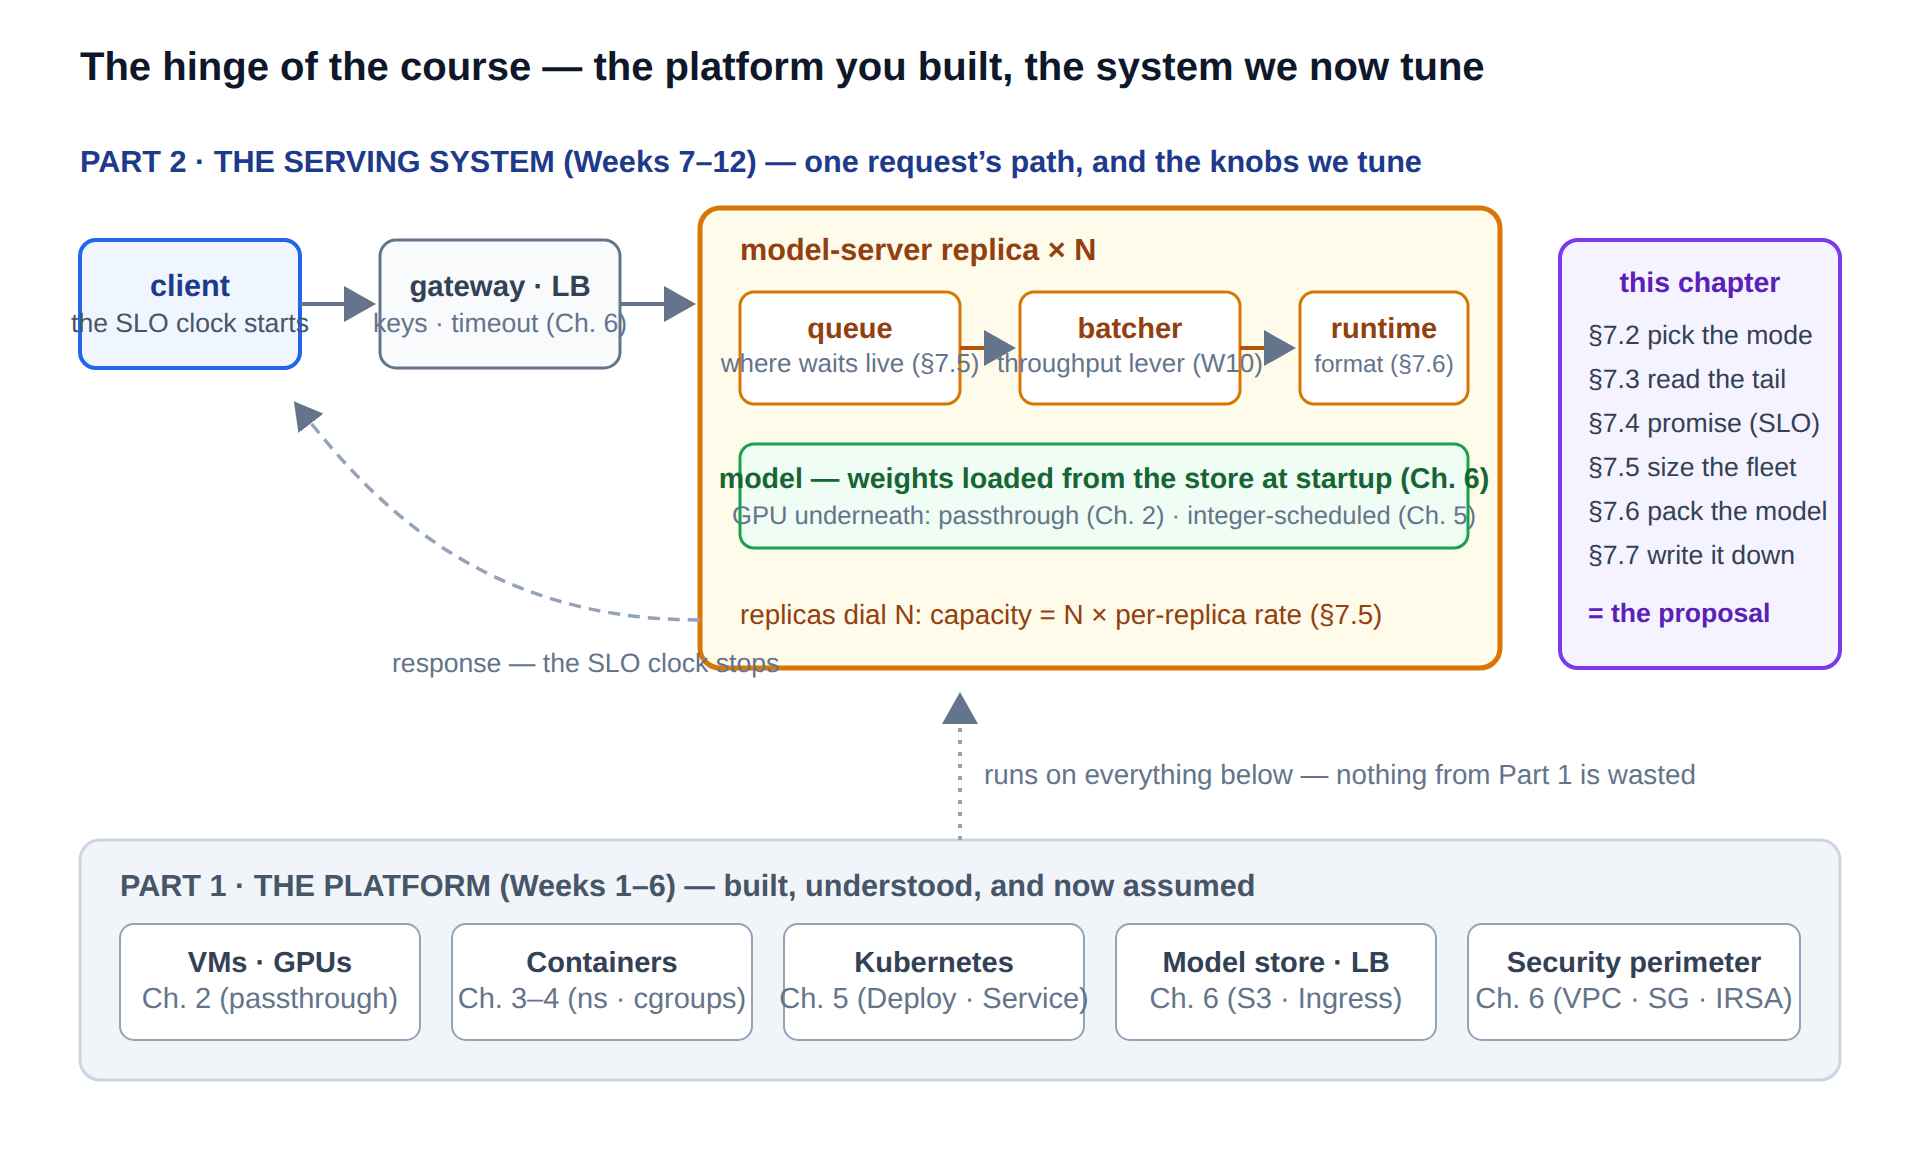
\includegraphics{figures/fig7-1_hinge.png}}\\[3pt]
  \figcaption{그림 7-1  강의의 경첩. 파트 1은 선 아래의 플랫폼을 만들었고 파트 2는 선 위의 서빙 시스템을 조정한다. 이 장의 각 절은 요청 경로에 방식(§7.2), 꼬리(§7.3), 약속(§7.4), 플릿(§7.5), 형식(§7.6), 제안서(§7.7)를 표시한다.}
\end{tbbfigure}

이번 주는 팀 프로젝트의 첫 제출물인 제안서 주간이기도 하다(§7.7). 행정적인 우연이 아니다. 제안서는 사례 7-A의 팀이 답하지 못한 질문에 숫자로 답하는 한 페이지 문서다. 무엇을 서빙하고(§7.6의 산출물), 어느 방식으로(§7.2), 무엇을 약속하며(§7.4의 SLO), 어느 부하에서 어떤 플릿(§7.5)을 사용하고, 월 비용 상한은 얼마인가(제1장의 비용 관점)? 여기서 §7.7까지의 모든 내용이 이 빈칸을 채울 재료다. 이 장 자체가 말 그대로 과제다.

\subsection*{이 장의 어휘}

\begin{tbbtablewrap}
  \begin{tabular}{@{}>{\raggedright\arraybackslash}m{\dimexpr 0.2660\tbltextwidth-2\tabcolsep\relax} >{\raggedright\arraybackslash}m{\dimexpr 0.7340\tbltextwidth-2\tabcolsep\relax}@{}}
  \arrayrulecolor{tbbnavy}\specialrule{1pt}{0pt}{0pt}
  \rowcolor{tbbtablehead}{\centering \bfseries\color{tbbnavy}용어} & {\centering \bfseries\color{tbbnavy}의미} \\
  \arrayrulecolor{tbbnavy}\specialrule{0.7pt}{0pt}{2pt}
  {\textbf{온라인 / 배치 / 스트리밍}} & {"누가 기다리는가"에 따라 나눈 세 가지 추론 방식. 요청마다 한 사람 / 아무도 없음 / 결과가 흐르는 모습을 지켜보는 사람으로 구분한다(§7.2).} \\
  \arrayrulecolor{tbbtableborder}\hline
  {\textbf{백분위수(pN)}} & {요청의 N\%가 이 값 이하로 빨랐음을 나타내는 지연 시간. p99는 가장 운 나쁜 1\%의 경험이며, 매일 나타나는 실제 사용자 집단이다.} \\
  \arrayrulecolor{tbbtableborder}\hline
  {\textbf{규모에서의 꼬리}} & {Dean과 Barroso의 관찰. 팬아웃에서는 드문 느림이 흔해진다. 1\% 느린 말단 100곳으로 팬아웃하면 요청의 63\%가 느려진다(§7.3).} \\
  \arrayrulecolor{tbbtableborder}\hline
  {\textbf{협조적 누락}} & {대표적인 부하 테스트 버그. 폐쇄 루프(closed loop) 시험기가 서버가 멈춘 동안 요청 전송도 멈춘 뒤, 멈춤을 제외한 백분위수를 보고한다(§7.3).} \\
  \arrayrulecolor{tbbtableborder}\hline
  {\textbf{SLI}} & {서비스 수준 지표(Service Level Indicator). "게이트웨이에서 500 ms 미만인 요청의 비율"처럼 신중하게 정의한 측정값으로, 현재 무슨 일이 일어나는지 나타낸다(§7.4).} \\
  \arrayrulecolor{tbbtableborder}\hline
  {\textbf{SLO}} & {서비스 수준 목표(Service Level Objective). 명시한 부하와 기간에 대해 스스로 정한 목표로, 우리 자신에게 하는 약속이다(§7.4).} \\
  \arrayrulecolor{tbbtableborder}\hline
  {\textbf{SLA}} & {서비스 수준 협약(Service Level Agreement). 비용이 걸린 외부 계약이며 항상 SLO보다 느슨하다(§7.4).} \\
  \arrayrulecolor{tbbtableborder}\hline
  {\textbf{오류 예산(error budget)}} & {1 − SLO 목표값으로 계산한, 쓸 수 있는 신뢰성 저하분. 30일 동안 99.9\%면 \textasciitilde{}43분이다. 성적표가 아니라 출시·동결 정책이다(§7.4).} \\
  \arrayrulecolor{tbbtableborder}\hline
  {\textbf{λ, W, L}} & {도착률(req/s), 시스템에 머무는 시간(s), 처리 중인 수. 안정적인 모든 시스템에서 Little's Law인 L = λ·W로 연결된다(§7.5).} \\
  \arrayrulecolor{tbbtableborder}\hline
  {\textbf{사용률 ρ · 여유분}} & {제공 부하 ÷ 용량. ρ → 1이면 지연 시간이 폭발하므로(하키 스틱) 온라인 플릿은 의도적으로 여유분을 구매한다(§7.5).} \\
  \arrayrulecolor{tbbtableborder}\hline
  {\textbf{서빙 가능한 산출물}} & {실제로 배포하는 가중치(safetensors), 구성 파일, 토크나이저다. 모델 스토어(제6장)에서 버전을 관리하며 런타임이 실행할 수 있는 형식이다(§7.6).} \\
  \arrayrulecolor{tbbnavy}\specialrule{1pt}{2pt}{0pt}
  \end{tabular}\par
  \figcaption{표 7-1  이 장에서 사용할 어휘}
\end{tbbtablewrap}

\begin{calloutbox}{tbbpurple}{tbbpurplefill}
{\normalsize\bfseries\color{tbbpurple}생각해 보기}\par\vspace{3pt}
\begin{tbbitemize}
  \item 사례 7-A를 좋아하는 실제 서비스의 규모로 재현해 보자. p99.9 = 5 s이고 하루 5,000만 건의 요청을 처리한다면 5초짜리 경험은 매일 몇 번 발생하는가? "p99.9"가 여전히 예외인가?
  \item 엔지니어의 대시보드는 평균을 그렸기 때문에 초록색이었다. 대신 그려야 할 두세 개 선과 경보 임계값을 어디서 가져올지 그려 보자. §7.4를 처음부터 설계한 뒤 읽고 답을 확인하자.
  \item 사례 7-B의 오류 행은 "0.4\% (23× 504, 17× 502)"다. 제6장의 상태 코드 현장 안내서에 따르면 두 코드 가운데 로드 밸런서가 자기 문제를 자백하는 것은 무엇이고, 서버를 탓하는 것은 무엇인가? §7.4의 SLO가 둘 다 세어야 하는 이유는 무엇인가?
\end{tbbitemize}
\end{calloutbox}

\section{세 가지 추론 방식: 누가 무엇을 기다리는가?}

제안서의 첫 번째 빈칸은 채우기는 가장 쉽지만 틀리면 가장 비싸다. 프레임워크나 GPU를 논하기 전에 한 가지 질문이 서빙 시스템의 형태를 결정한다. \textbf{누가 이 추론에서 무엇을 기다리는가?} 한 사람이 \textit{이} 답을 기다리는 온라인, 아무도 기다리지 않는 배치, 한 사람이 답이 \textit{흐르는} 모습을 지켜보는 스트리밍이라는 세 답은 모델 가중치가 바이트 단위로 같더라도 운영 설명서를 거의 공유하지 않을 만큼 다른 시스템을 만든다(그림 7-2).

\begin{tbbfigure}
  \adjustbox{max width=0.94\linewidth,max totalheight=0.46\textheight}{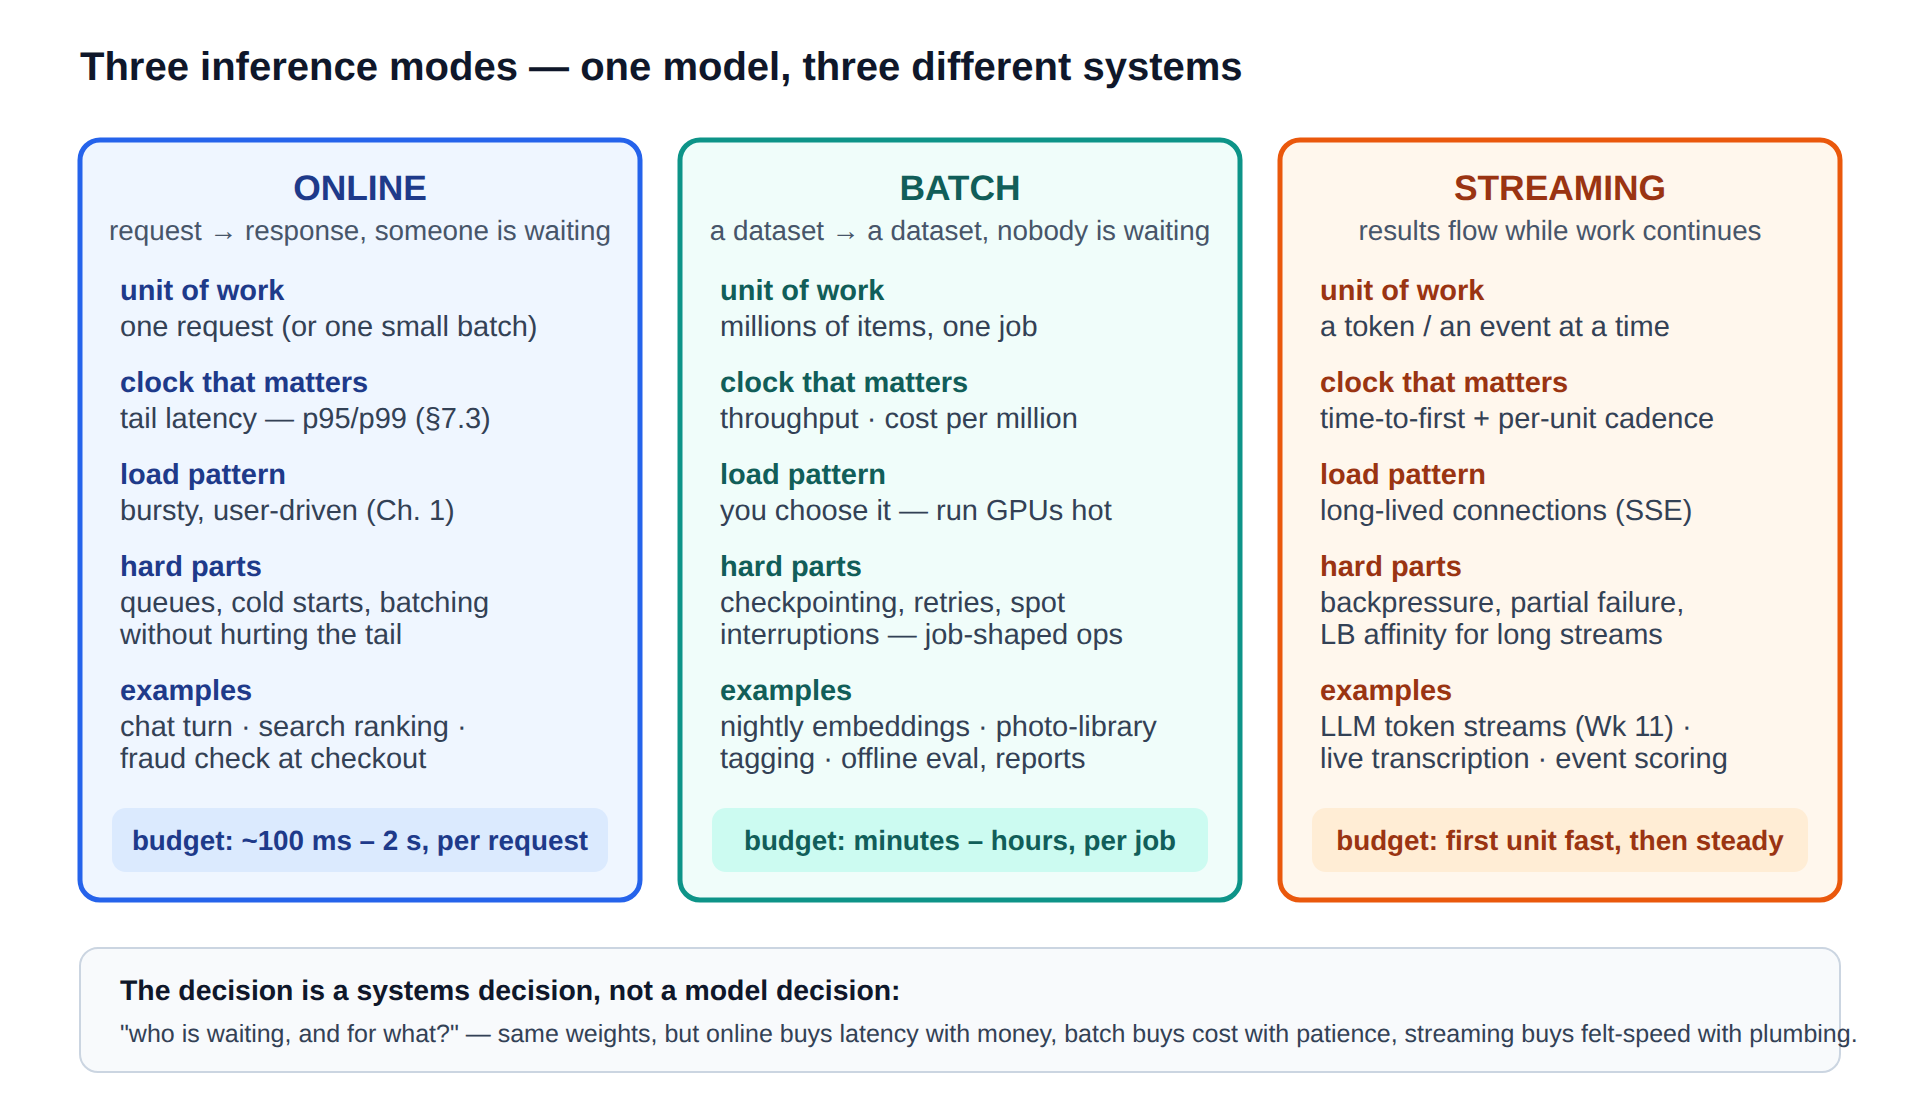
\includegraphics{figures/fig7-2_modes.png}}\\[3pt]
  \figcaption{그림 7-2  세 가지 추론 방식. 같은 모델로 만든 세 시스템에서 온라인은 꼬리를, 배치는 비용을, 스트리밍은 빠르다는 느낌을 관리한다.}
\end{tbbfigure}

\subsection*{온라인: 모두가 가정하는 기본값이자 이 강의가 가장 엄격하게 다룰 방식}

\textbf{온라인 추론}은 사람 또는 비용을 지불하는 상위 서비스가 기다리는 동안 실시간 요청에 응답한다. 대화의 한 차례, 검색 순위 결정, 결제 흐름의 사기 탐지가 예다. 이 방식의 물리는 다음과 같다. 작업 단위는 요청 하나다. 사용자가 실제로 이탈하는 곳이 꼬리이므로 중요한 시계는 지연 시간 분포의 \textbf{꼬리}다(§7.3). 부하는 사용자가 원하는 때 도착해 버스트를 보인다(제1장). 따라서 수요보다 \textit{먼저} 용량을 프로비저닝해야 한다. 사례 1-A의 대기열 붕괴부터 12주 차 오토스케일링까지 모두 이 방식에서 다루는 이유다. 이 책에서 수식어 없이 "서빙"이라 하면 온라인을 뜻한다. 꼬리와 절충하는 배치 처리, 콜드 스타트, SLO, 플릿 규모 산정 같은 파트 2의 어려운 주제가 모두 제값을 하는 방식이다.

\subsection*{배치: 쉬운 방식 — 언제나 먼저 검토하자}

\textbf{배치 추론}은 아무도 기다리지 않는 상태에서 데이터셋에 모델을 실행한다. 오늘 업로드된 모든 사진에 밤새 태그를 붙이고, 매주 일요일 문서 말뭉치를 다시 임베딩하며, 회의 전에 지난 분기 청구 건의 점수를 매긴다. 제1장에서 말한 "학습 형태의 서빙"이다. 배치 추론이 등장하면서 미뤄 둔 질문에 답할 수 있다. 제1장의 생각해 볼 문제는 \textit{무엇이 단순해지는가}를 물었다. 솔직하고 다소 민망한 목록은 다음과 같다. 꼬리 SLO가 \textbf{사라진다.} 야간 작업의 p99를 경험하는 사람은 없고 마감 시각만 중요하다. 오토스케일링도 \textbf{사라진다.} 직접 부하를 정하므로 뒤쫓아야 할 뜻밖의 상황이 없다. §7.5의 하키 스틱은 적이 아니라 친구가 된다. 기다리는 사람이 없으므로 온라인 원칙과 정반대로 GPU를 의도적으로 95\% 이상 사용률로 돌린다. 실패의 비용은 사용자가 아니라 재시도이므로 크게 할인되는 중단 가능 용량인 \textbf{스팟 인스턴스(spot instance)}(12주 차)가 배치에 완벽히 맞는다. 남는 것은 진행 상태 체크포인트, 멱등 재시도, \textbf{백만 항목당 비용}이라는 단일 지표를 중심으로 한 작업 형태의 엔지니어링이다.

여기서 얻는 실용적인 원칙이 있다. \textbf{세상에서 가장 저렴한 지연 시간 최적화는 실제로는 아무도 기다리지 않았음을 발견하는 것이다.} "이 답이 한 시간 뒤에 와도 괜찮은가?"라고 물으면 "실시간 추론이 필요하다"는 요구사항 가운데 놀랄 만큼 많은 것이 사라진다. 온라인에서 배치로 옮기는 모든 워크로드는 SLO 엔지니어링을 예약 작업으로 바꾼다. 제안서에는 트래픽 가운데 실제로 온라인인 부분을 명시하고 나머지는 쉬운 방식으로 보내야 한다.

\subsection*{스트리밍: 배관으로 빠르다는 느낌을 산다}

\textbf{스트리밍 추론}은 작업이 계속되는 동안 결과를 전달한다. 대화 화면을 살아 있는 것처럼 느끼게 하는 LLM 토큰 스트림이 가장 유명하지만 실시간 음성 전사와 이벤트 채점도 포함된다. 시계는 둘로 나뉜다. 첫 결과가 나타날 때까지의 시간인 \textbf{첫 단위 도착 시간}이 새로운 "지연 시간"이 되고, 이후에는 초당 단위 수를 나타내는 \textbf{전송 속도}가 중요하다. 기술만큼 심리적인 기법이다. 마지막 토큰이 8초에 도착해도 첫 토큰이 300 ms에 왔다면 답이 \textit{빠르게 느껴진다.} 그래서 11주 차에는 첫 토큰 도착 시간을 일급 SLI로 다룬다. 대가는 배관이다. 버퍼링 없이 제6장의 모든 프록시와 로드 밸런서를 통과해야 하는 SSE 또는 WebSocket 장기 연결, 소비자가 생산자보다 느릴 때의 \textbf{역압(backpressure)}, 답의 절반이 이미 전송된 상태에서 "재시도"의 의미를 정하는 부분 실패 의미 체계가 필요하다. 여기서는 방식의 이름만 소개하고 서빙 엔진 내부는 11주 차에 다룬다.

\begin{tbbtablewrap}
  \begin{tabular}{@{}>{\raggedright\arraybackslash}m{\dimexpr 0.2606\tbltextwidth-2\tabcolsep\relax} >{\raggedright\arraybackslash}m{\dimexpr 0.2447\tbltextwidth-2\tabcolsep\relax} >{\raggedright\arraybackslash}m{\dimexpr 0.2394\tbltextwidth-2\tabcolsep\relax} >{\raggedright\arraybackslash}m{\dimexpr 0.2553\tbltextwidth-2\tabcolsep\relax}@{}}
  \arrayrulecolor{tbbnavy}\specialrule{1pt}{0pt}{0pt}
  \rowcolor{tbbtablehead}{\centering \bfseries\color{tbbnavy}질문} & {\centering \bfseries\color{tbbnavy}온라인} & {\centering \bfseries\color{tbbnavy}배치} & {\centering \bfseries\color{tbbnavy}스트리밍} \\
  \arrayrulecolor{tbbnavy}\specialrule{0.7pt}{0pt}{2pt}
  {\textbf{누가 기다리는가?}} & {요청마다 사람 / 실시간 상위 서비스} & {아무도 없음, 기껏해야 마감 시각} & {결과가 흐르는 모습을 보는 사람} \\
  \arrayrulecolor{tbbtableborder}\hline
  {\textbf{시계}} & {꼬리 지연 시간(p95/p99)} & {작업 완료 · 백만 항목당 비용} & {첫 결과 도착 시간 + 이후 전송 속도} \\
  \arrayrulecolor{tbbtableborder}\hline
  {\textbf{부하 패턴}} & {사용자가 결정(버스트)} & {운영자가 결정(일정)} & {장기 연결, 세션 형태} \\
  \arrayrulecolor{tbbtableborder}\hline
  {\textbf{사용률 자세}} & {의도적인 여유분(§7.5)} & {의도적으로 뜨겁게 실행(ρ→0.95)} & {여유분 + 연결 예산} \\
  \arrayrulecolor{tbbtableborder}\hline
  {\textbf{실패 비용}} & {즉시 영향을 받는 사용자} & {보이지 않는 재시도} & {문장 중간에 끊긴 스트림} \\
  \arrayrulecolor{tbbnavy}\specialrule{1pt}{2pt}{0pt}
  \end{tabular}\par
  \figcaption{표 7-2  방식을 결정하는 다섯 가지 질문}
\end{tbbtablewrap}

마지막으로 현실을 인정하자. 실제 제품은 \textbf{혼합물}이다. 대화형 제품은 답을 스트리밍하고, 매일 밤 검색용 임베딩을 미리 계산하며(배치), 요청 경로 안에서 후보 문서의 순위를 정한다(온라인). 따라서 제안서 양식은 확인란 하나가 아니라 트래픽 \textit{분해}를 요구한다. 검토자는 이 분해를 보고 팀이 실제로 시스템을 고민했는지 처음 판단한다.

\begin{calloutbox}{tbbpurple}{tbbpurplefill}
{\normalsize\bfseries\color{tbbpurple}생각해 보기}\par\vspace{3pt}
\begin{tbbitemize}
  \item 팀이 "홈페이지에 필요하므로 추천 모델은 반드시 온라인이어야 한다"고 말한다. 홈페이지는 사용자마다 세션당 최대 한 번 렌더링되고 프로필은 하루에 한 번 바뀐다. 배치 재설계를 옹호해 보자. 무엇을 미리 계산하고, 남는 작은 온라인 구성 요소가 있다면 무엇이며, SLO는 어떻게 바뀌는가?
  \item LLM 대화형 제품에서 대화가 즉각적이라고 느껴질 때와 고장 났다고 느껴질 때를 가르는 두 스트리밍 시계, 즉 첫 토큰 도착 시간과 초당 토큰 수를 적어 보자. 사용하는 대화형 서비스에서 초시계로 숫자를 추정해 직관을 확인하자.
  \item 반드시 오전 6시까지 끝나야 하는 야간 작업은 어느 방식인가? 항목별 지연 시간 목표는 없지만 마감 시각은 있다. 그렇다면 "아무도 기다리지 않는다"는 말이 완전히 맞는가? 이 작업의 SLO 형태 문장은 무엇인가? §7.4의 어휘를 사용해 작성하자.
\end{tbbitemize}
\end{calloutbox}

\section{지연 시간은 분포다 — 꼬리 읽기}

사례 7-B는 이미 기습적으로 논지를 보여 주었다. 이 절에서는 이를 규율로 만든다. 백분위수가 붙지 않은 지연 시간 숫자는 정보가 아니라 사례 7-A가 일어나기를 기다리는 상태다. 그림 7-3을 정신 모형으로 기억하자. 모든 서비스의 지연 시간은 긴 꼬리가 있는 \textbf{오른쪽으로 치우친 분포}다. 분포를 읽는 법, 증폭되는 방식, 도구가 거짓말하는 방식을 다루는 아래 세 가지 사실은 서빙 시스템 운영자의 실무 지식이다.

\begin{tbbfigure}
  \adjustbox{max width=0.94\linewidth,max totalheight=0.46\textheight}{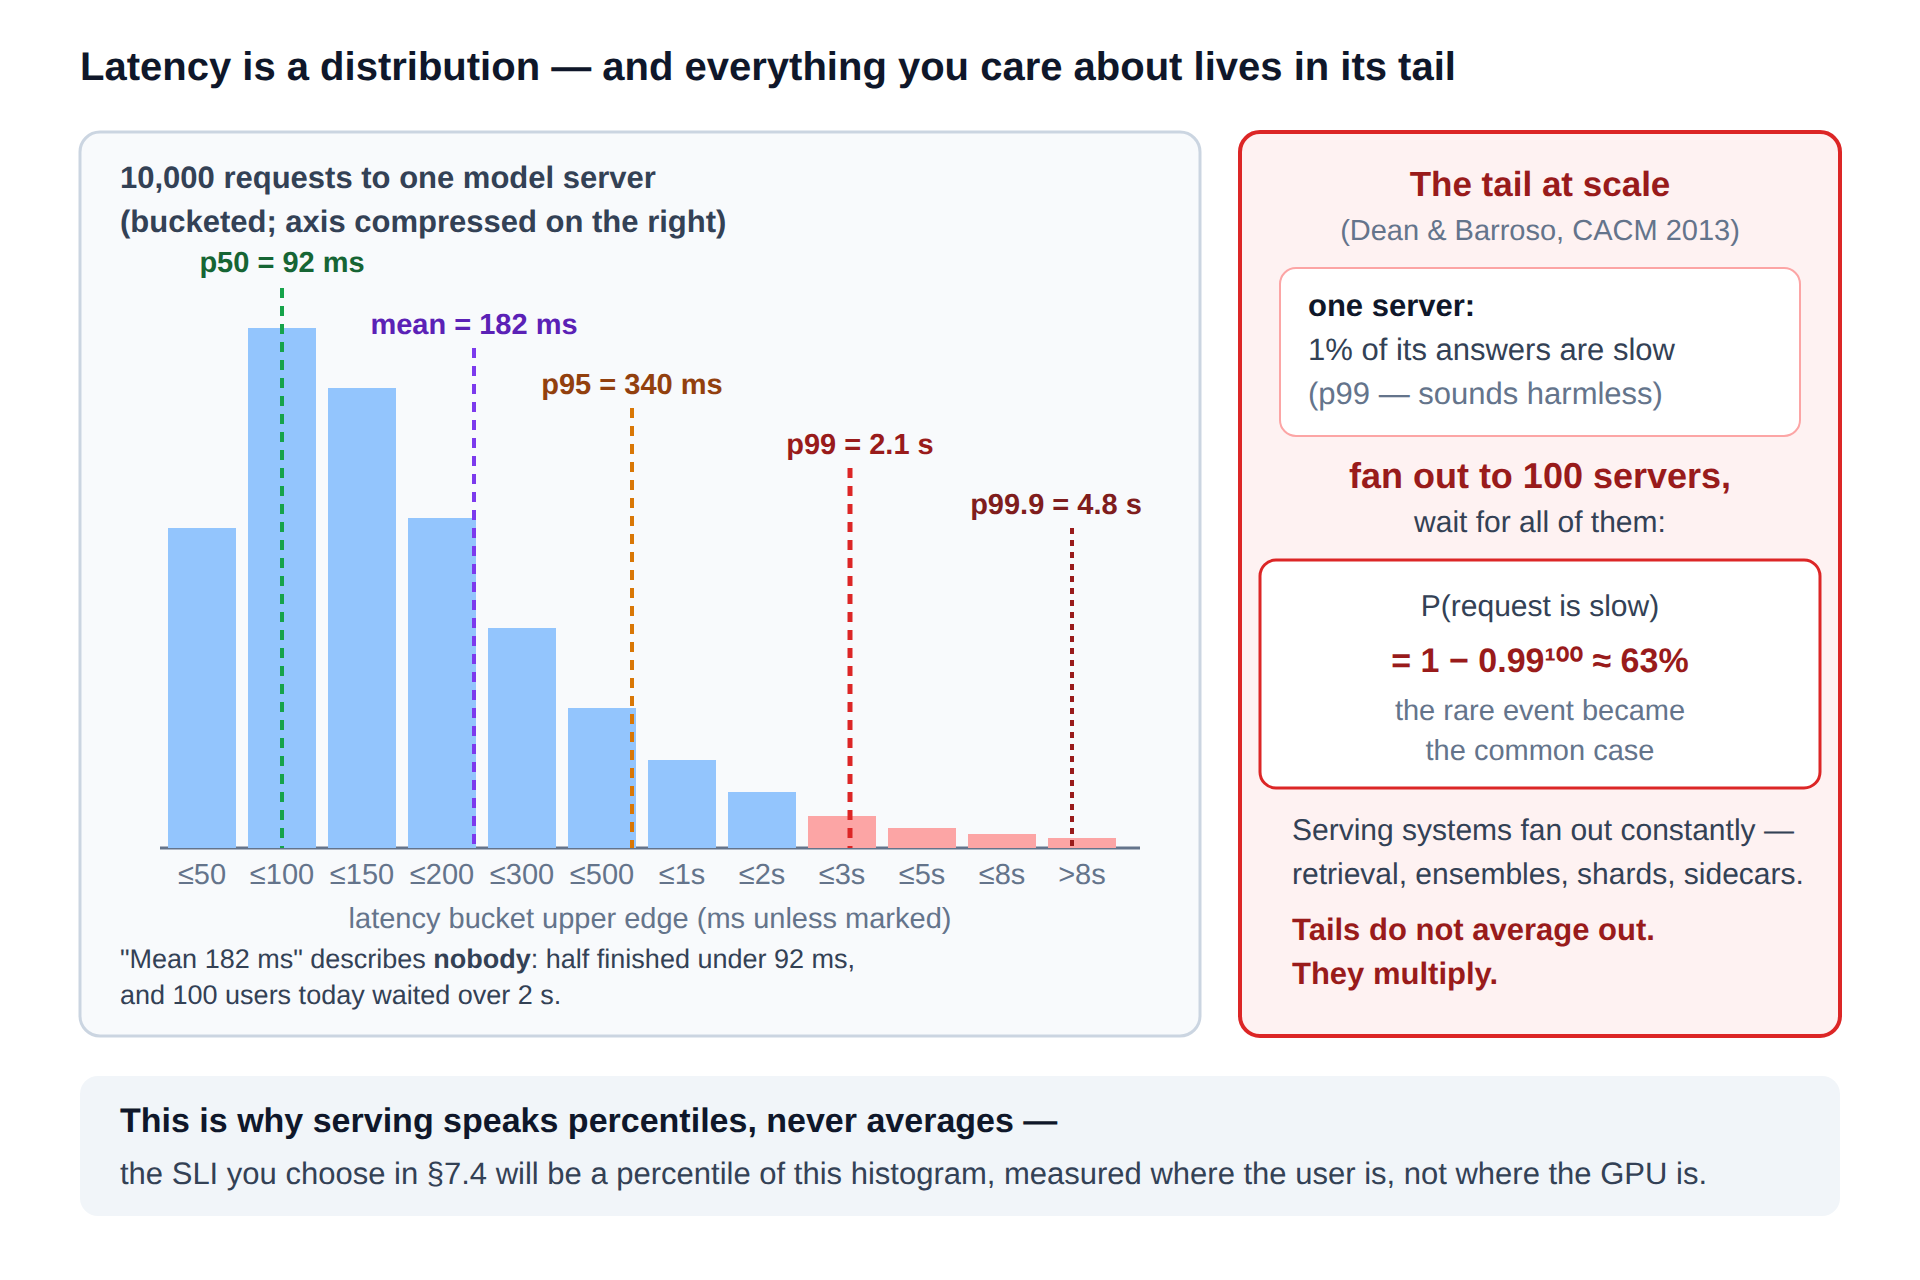
\includegraphics{figures/fig7-3_tail.png}}\\[3pt]
  \figcaption{그림 7-3  사례 7-B 뒤의 지연 시간 분포와 백분위수 표시. 오른쪽은 팬아웃에서 드문 느림을 흔한 경험으로 바꾸는 규모에서의 꼬리 계산이다.}
\end{tbbfigure}

\subsection*{백분위수 문법}

\textbf{pN은 요청의 N\%가 더 빠르게 끝난 지연 시간이다.} p50(중앙값)은 일반적인 경험이고 p95와 p99는 운 나쁜 5\%와 1\%이며 p99.9는 CEO가 전사 회의 데모에서 뽑는 집단이다. 네 가지 문법 규칙이 정직함을 지켜 준다. 첫째, \textbf{평균은 백분위수가 아니며} 치우친 분포에서는 아무도 설명하지 못한다. 꼬리에 끌려 올라가면서도 꼬리 크기에 관해서는 아무 말도 하지 않는다. 사례 7-B의 평균 182 ms는 p50과 p90 사이에 놓였지만 누구도 경험하지 않았다. 둘째, \textbf{백분위수는 기간과 모집단의 속성}이다. \textit{어디서, 어느 기간, 어느 부하에서 측정했는지} 없으면 "p99 = 2.1 s"는 아무 의미가 없다. 화요일 아침 p99와 블랙프라이데이 p99는 서로 다른 사실이다. 셋째, \textbf{백분위수는 더할 수 없다.} 단계 A와 B가 각각 p99 = 100 ms라도 파이프라인 p99는 \textit{200 ms가 아니다.} A와 B에서 운 나쁜 1\%는 대부분 서로 다른 요청이다. 파이프라인 p99는 그 사이 어딘가에 있으며 전체 분포만 위치를 알려 줄 수 있다. 넷째, 운영상 따라오는 결론으로 \textbf{백분위수를 평균할 수 없다.} 레플리카 10개의 p99 평균은 플릿 p99가 아니다. 레플리카나 시간 전체를 집계하려면 \textit{히스토그램(histogram)}을 합쳐야 한다. 그래서 진지한 지표 시스템(14주 차 Prometheus)은 미리 계산한 백분위수가 아니라 히스토그램 버킷으로 지연 시간을 전송한다.

\subsection*{규모에서의 꼬리: 증폭되는 드문 느림}

실무자가 p50보다 p99에 집착하는 이유는 무엇일까? "꼬리에서 사용자가 이탈한다"는 이유 외에 구조적인 증폭기가 있다. 모든 서빙 엔지니어가 결국 읽게 되는 Dean과 Barroso의 \textbf{"The Tail at Scale"}(CACM, 2013)에 이름이 붙어 있다. 현대 서빙은 팬아웃한다. 사용자 요청 하나가 검색 샤드, 임베딩 서비스, 순위 결정기, 안전 필터, 템플릿 렌더러를 거친다. 각 하위 호출이 1\%만 느리다고 하자(p99 오동작). 이런 호출 100개로 팬아웃해 모두 기다리면 사용자 요청이 느린 호출을 하나 이상 만날 확률은 1 − 0.99¹⁰⁰ ≈ \textbf{63\%}다. 각 구성 요소의 \textit{드문} 사건이 사용자의 \textit{흔한} 경험으로 바뀐다. 꼬리는 평균으로 사라지지 않고 증폭된다. 이 계산 하나가 서빙 아키텍처의 한 계열을 설명한다. 팬아웃을 얕게 유지하고, 호출별 타임아웃을 사용자 마감 시각보다 짧게 설정하며(제6장의 게이트웨이 규율), 논문에서 유명해진 \textbf{헤지 요청}을 사용한다. 일정 시간이 지나면 같은 질의를 두 번째 레플리카에 보내 먼저 온 답을 택함으로써 서버 하나의 꼬리를 둘의 \textit{최솟값}으로 바꾼다. 헤지는 중복 작업을 꼬리 지연 시간과 맞바꾼다. 다시 서빙 삼각형이며 비용을 써서 꼬리를 산다.

\subsection*{부하 테스트가 거짓말하는 방식: 협조적 누락}

백분위수는 측정 도구만큼만 정직하다. 업계에서 가장 흔한 측정 버그에는 알아 둘 만한 이름이 있다. Gil Tene가 이름 붙이고 HdrHistogram과 wrk2를 만들어 해결한 \textbf{협조적 누락(coordinated omission)}이다. 버그는 다음과 같다. \textit{폐쇄 루프} 부하 시험기는 처리 중인 요청 수를 고정한다. 각 가상 사용자가 요청을 보내고 응답을 기다린 뒤 다시 보낸다. 서버가 멈추면 시험기의 가상 사용자도 모두 기다리므로, 시험기는 \textit{서버가 최악인 바로 그때 정중하게 부하 생성을 멈춘다.} 그런 다음 우연히 보낸 요청만으로 백분위수를 계산해 보고한다. 데이터에는 멈춤이 거의 나타나지 않는다. 실제 사용자는 그렇게 정중하지 않다. 서버가 멈춘 동안에도 계속 도착하며 실제 대기 시간에는 멈춤도 포함된다. 터미널 기록 7-1은 의도적으로 조작한 서버에서 그 차이를 보여 준다.

\begin{terminalbox}
\begin{Verbatim}[breaklines=true,breakanywhere=true,fontsize=\small,formatcom=\color{tbbtermfg},codes=\tbbcodeactive]
# the server is rigged to stall 1.5 s every 60 s (a "GC pause")
$ wrk -t4 -c64 -d120s http://svc/predict      # closed loop, 64 in flight
  Latency   p50 11ms    p99 13ms    max 1.51s
# during each stall only the 64 in-flight requests wait; 64 samples out
# of ~60,000/window = 0.1% -> the p99 never sees the stall. "all green."
$ wrk2 -t4 -c64 -R1000 -d120s http://svc/predict   # open loop: 1,000/s,
  Latency   p50 12ms    p99 1,140ms p99.9 1.49s    # arrivals never pause
# 1,500 requests' worth of demand arrived DURING each stall and queued.
# wrk2 charges the server for the wait, as a user's clock would.
\end{Verbatim}
\end{terminalbox}
\figcaption{터미널 기록 7-1  협조적 누락 시연. 같은 서버와 같은 멈춤에서 폐쇄 루프 도구는 p99 = 13 ms를, 개방 루프 도구는 p99 = 1.14 s를 보고한다. 둘 중 하나만 사용자를 설명한다.}

교훈은 "wrk는 나쁘고 wrk2는 좋다"가 아니다. \textbf{부하 생성기는 도착 과정을 모델링}하므로 현실과 맞는 모델을 골라야 한다는 것이다. 동시성을 고정하는 폐쇄 루프는 "클라이언트가 차례를 기다릴 때 이 서버가 얼마나 감당할 수 있는가?"에 답한다. 용량 탐색에는 좋은 질문이다. wrk2의 -R이나 Locust의 고정 처리량 방식처럼 도착률을 고정하는 개방 루프(open loop)는 "초당 λ건의 요청이 올 때 사용자는 무엇을 경험하는가?"에 답한다. 실제 도착은 예의상 멈추지 않으므로 SLO에 맞는 질문이다. 9주 차 실습에서는 Locust로 프레임워크가 서빙하는 모델을 부하 테스트하며 개방 루프 답을 요구한다. 15주 차 데모도 이를 기준으로 평가한다.

\begin{calloutbox}{tbbpurple}{tbbpurplefill}
{\normalsize\bfseries\color{tbbx5B21B6}상자 7-1  부하 테스트 위생 — 숫자가 통과해야 할 체크리스트}\par\vspace{3pt}
\begin{tbbitemize}
  \item \textbf{먼저 워밍업하고 별도로 보고한다.} 첫 요청은 모델 로드, CUDA 컨텍스트, JIT, 캐시 같은 일회성 비용을 낸다. 제2장 실습에서 측정했다. 정상 상태 백분위수는 워밍업 뒤부터 시작하며 워밍업 자체는 콜드 스타트 데이터다(12주 차).
  \item \textbf{SLO 질문에는 개방 루프를 사용한다.} 목표 λ와 그 이상에서 도착률을 고정한다. 폐쇄 루프는 용량 탐색에만 사용하고 그렇게 표시한다.
  \item \textbf{꼬리를 채울 만큼 오래 실행한다.} 100 req/s에서 p99.9는 10초마다 요청 하나다. 30초 테스트에는 표본이 약 3개뿐이다. 초가 아니라 분 단위로 실행한다.
  \item \textbf{오류와 지연 시간을 반드시 함께 보고한다.} 요청의 5\%를 타임아웃하는 서버는 살아남은 요청만 보면 훌륭한 p99를 보인다. 사례 7-B가 같은 카드에 오류율을 인쇄한 이유다. 타임아웃은 트렌치코트를 입은 꼬리다.
  \item \textbf{사용자 위치에서 측정한다.} 파드 내부가 아니라 제6장의 게이트웨이를 통과한 클라이언트 쪽에서 측정한다. 놓치기 가장 쉬운 대기열은 자기 서버 앞에 있는 대기열이다.
  \item \textbf{최소 한 번 반복한다.} 실행마다 3배 움직이는 백분위수는 서버가 아니라 테스트에 관해 말하고 있다.
\end{tbbitemize}
\end{calloutbox}

\vspace{3.0pt}

\begin{calloutbox}{tbbpurple}{tbbpurplefill}
{\normalsize\bfseries\color{tbbpurple}생각해 보기}\par\vspace{3pt}
\begin{tbbitemize}
  \item 파이프라인이 게이트웨이 → 검색 → 모델 → 후처리로 이어지고 각각 p99 = 100 ms다. 팀원이 "전체 p99 ≈ 400 ms"로 예산을 잡았다. 이 문장의 서로 다른 오류 두 가지, 즉 백분위수를 더하는 문제와 파이프라인 꼬리를 지배하는 요소에 관한 문제를 설명하고, 정직한 예산을 위해 필요한 데이터를 말하자.
  \item 프로젝트에서 예상되는 팬아웃(검색 + 모델 + 안전 필터 = 호출 3개)의 규모에서의 꼬리를 계산하자. 각각 1\%가 느리다면 느린 호출을 만나는 사용자 요청 비율은 얼마인가? 팬아웃이 얼마일 때 10\%를 넘는가?
  \item 간단한 서버의 sleep()과 부하 도구 두 번 실행만으로 협조적 누락을 60초 동안 시연하는 방법을 설계하자. 각 실행이 어떤 숫자를 보고할 것으로 예상하는가? 그런 다음 실제로 실행하자. 이 장의 실습 선택지 가운데 하나다.
\end{tbbitemize}
\end{calloutbox}

\section{SLI, SLO, SLA와 오류 예산}

수요일 아침 CTO의 지시인 \textit{"고객에게 무엇을 약속했는가? 그 문제부터 해결하라"}에는 실전에서 검증된 표준 해결책이 있다. 이 강의는 이를 발명한 Google의 Site Reliability Engineering 규율에서 그대로 가져온다. SRE 책 제4장이 이번 주 필독 자료다. 해결책은 자주 혼동되지만 절대 그래서는 안 되는 세 단어의 작은 사다리인 \textbf{SLI, SLO, SLA}다(그림 7-4). 이 사다리를 한 번 익히면 사례 7-A는 구조적으로 불가능해진다. 논쟁에 참여한 사람마다 서로 다른 단이 빠져 있었다.

\begin{tbbfigure}
  \adjustbox{max width=0.94\linewidth,max totalheight=0.46\textheight}{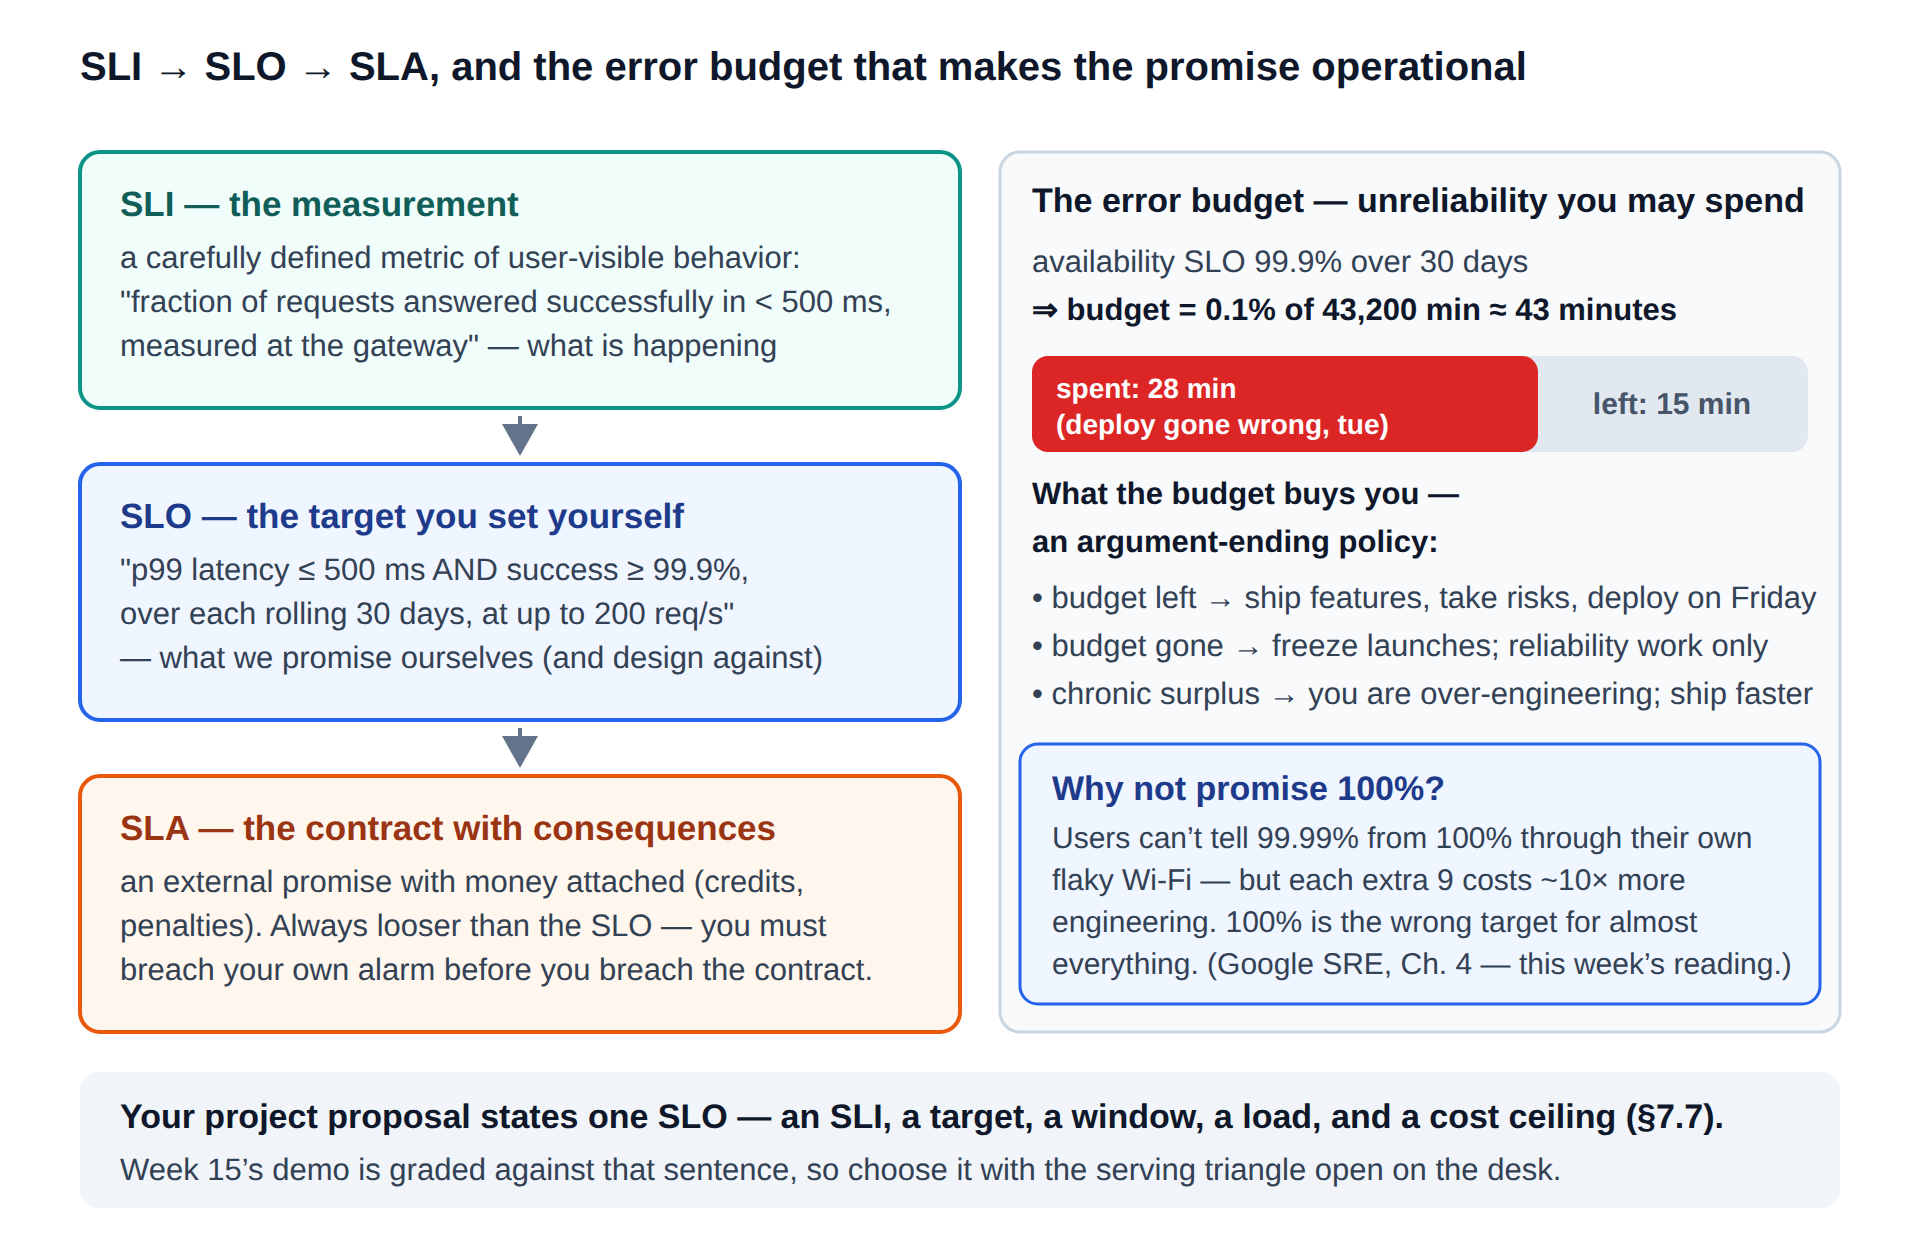
\includegraphics{figures/fig7-4_slo.png}}\\[3pt]
  \figcaption{그림 7-4  사다리와 예산. SLI는 측정하고 SLO는 목표를 정하며 SLA는 계약한다. 오류 예산은 목표를 정책 기계로 바꾼다.}
\end{tbbfigure}

\subsection*{SLI: 사용자처럼 측정하고 회계사처럼 센다}

\textbf{서비스 수준 지표(Service Level Indicator)}는 사용자에게 보이는 동작을 신중하게 정의한 측정값이다. 기술은 정의에 있다. 좋은 SLI는 (a) \textbf{사용자와 가까워야} 한다. 파드 내부가 아니라 사용자가 있는 게이트웨이 또는 그 너머에서 측정해야 한다. 서버 앞 대기열은 내부에서 보이지 않는다는 §7.3의 위생 규칙이다. (b) \textbf{좋은 이벤트 수를 전체 이벤트 수로 나눈 비율}이어야 한다. 비율은 기간에 걸쳐 합성할 수 있고 트래픽 변화에도 견딘다. "평균 지연 시간"이 아니라 "500 ms 안에 성공적으로 응답한 요청의 비율"을 쓴다. (c) \textbf{논쟁 없이 셀 수 있어야} 한다. 엔지니어 두 명이 정의를 읽고 같은 숫자를 내야 한다. 사례 7-A의 대시보드는 세 조건을 동시에 어겼다. 비율이 아닌 평균을 그렸고, 사용자와 가까운 곳이 아닌 서버 쪽에서 계산했으며, 성공만 포함해 논쟁의 여지를 남겼다. 표 7-3은 추론 서비스에 사용할 수 있는 선택지다.

\begin{tbbtablewrap}
  \begin{tabular}{@{}>{\raggedright\arraybackslash}m{\dimexpr 0.2287\tbltextwidth-2\tabcolsep\relax} >{\raggedright\arraybackslash}m{\dimexpr 0.4362\tbltextwidth-2\tabcolsep\relax} >{\raggedright\arraybackslash}m{\dimexpr 0.3351\tbltextwidth-2\tabcolsep\relax}@{}}
  \arrayrulecolor{tbbnavy}\specialrule{1pt}{0pt}{0pt}
  \rowcolor{tbbtablehead}{\centering \bfseries\color{tbbnavy}SLI 계열} & {\centering \bfseries\color{tbbnavy}잘 정의한 예} & {\centering \bfseries\color{tbbnavy}피하는 함정} \\
  \arrayrulecolor{tbbnavy}\specialrule{0.7pt}{0pt}{2pt}
  {\textbf{가용성}} & {게이트웨이에서 LB가 만든 502/504를 포함해 5xx가 아닌 상태로 응답한 요청의 비율} & {코드가 반환한 오류만 세는 함정. LB의 504도 사용자에게 보이는 실패다(제6장).} \\
  \arrayrulecolor{tbbtableborder}\hline
  {\textbf{지연 시간}} & {게이트웨이에서 500 ms 안에 완료된 성공 요청의 비율(동일한 표현: p99 ≤ 500 ms)} & {평균 계산, 파드 내부 측정, 지연 시간 집합에서 오류를 조용히 제외하는 함정(§7.3)} \\
  \arrayrulecolor{tbbtableborder}\hline
  {\textbf{품질(대리 지표)}} & {스키마·안전성 검증을 통과한 응답의 비율. 스트리밍은 끝까지 완료된 스트림의 비율} & {모델 \textit{정확도}를 SLO로 약속하는 함정. 정확도는 인프라가 아니라 세상의 변화에 따라 드리프트한다(14주 차 드리프트 모니터링).} \\
  \arrayrulecolor{tbbtableborder}\hline
  {\textbf{최신성(배치)}} & {야간 출력이 06:00 전에 완전히 도착한 아침의 비율} & {배치 작업에는 SLO가 전혀 없다고 보는 함정. §7.2의 마감 시각도 약속이다.} \\
  \arrayrulecolor{tbbtableborder}\hline
  {\textbf{비용(예산 지표)}} & {매주 SLIs 옆에 보고하는 요청 1,000개당 \$} & {비용을 SLI로 취급하는 함정. 비용은 요청별 약속이 아니라 보고하는 \textit{제약 조건}이다(제1장의 삼각형).} \\
  \arrayrulecolor{tbbnavy}\specialrule{1pt}{2pt}{0pt}
  \end{tabular}\par
  \figcaption{표 7-3  추론 서비스의 SLI 선택지와 각각의 함정}
\end{tbbtablewrap}

\subsection*{SLO: 기간과 부하 조항이 있는 선택한 지점}

\textbf{서비스 수준 목표(Service Level Objective)}는 명시한 기간 동안의 SLI 목표값이며 팀이 \textit{자기 자신}에게 약속하는 숫자다. 다섯 가지 필수 요소가 있는데 학생 제안서는 역사적으로 마지막 두 가지를 빼먹었다. \textbf{(1)} 참조할 SLI, \textbf{(2)} 목표값("500 ms 안에 처리한 요청이 99.5\% 이상" / "p99 ≤ 500 ms"), \textbf{(3)} 평가 기간("이동식 30일마다" — "한 시간 동안 나빴다"는 말을 논쟁이 아닌 산술로 바꾼다), \textbf{(4)} \textbf{부하 조항}("초당 최대 200건의 지속 부하")이 필요하다. §7.5에서 지연 시간이 부하의 함수임을 볼 것이므로 λ에 상한을 두지 않은 p99 약속은 아무것도 약속하지 않는다. 부하 조항 없는 SLO는 소망이다. \textbf{(5)} 이 강의에서 추가한 \textbf{비용 상한}("월 \$900 이하")도 필요하다. 제1장의 삼각형에서 빠름·대용량·저비용 가운데 둘은 비용을 지불해 셋째를 살 수 있다고 배웠으므로, 셋째 꼭짓점을 무시한 약속은 아직 엔지니어링 문장이 아니다.

목표 \textit{숫자}는 어디서 나오는가? 야심에서 나오지 않는다. 규율은 사용자가 개선을 더는 알아채지 못하는 지점인 \textbf{제품이 방어할 수 있는 가장 느슨한 SLO}를 고르는 것이다. 불필요하게 9 하나를 더할 때마다 아래에서 볼 엔지니어링 비용이 배로 늘어난다. 대화형 제품의 p99 800 ms는 충분히 방어할 수 있다. 결제 흐름 안의 사기 탐지는 주변 페이지가 더 엄격한 예산을 강제한다. 야간 배치에는 그런 예산이 전혀 없다. 숫자로 하는 제품 대화이며, 바로 \textit{지금} 제안서에서 나누는 것이 15주 차 데모를 사례 7-A와 가른다. 데모는 이번 주에 작성한 문장을 기준으로 평가한다.

\subsection*{오류 예산: 써도 되는 신뢰성 저하분}

SLO의 운영상 천재성은 여집합에 있다. 30일 동안 99.9\%를 약속하면 0.1\%인 약 \textbf{43분}은 \textit{사용해도 되는} 몫이며, 이를 \textbf{오류 예산}이라 한다. 이 관점 전환은 심리적·정치적으로 중요하다. 신뢰성이 "감히 금요일에 배포하다니" 같은 미덕 경쟁에서 자원 장부로 바뀐다. 예산이 남으면 기능을 출시하고 실험하며 자유롭게 배포한다. 예산은 속도를 위해 쓰라고 존재한다. 예산을 다 쓰면 출시를 동결하고 기간이 회복될 때까지 팀 시간을 신뢰성에 투입한다. 부사장의 기분이 아니라 \textit{사전 합의}에 따른다. 예산이 계속 남으면 과도하게 설계한 것이다. SLO를 느슨하게 하거나 더 빠르게 출시해야 한다. 예산은 사례 7-A의 논쟁도 반대 방향으로 끝낸다. PM이 불만을 상향 보고하면 답은 더 이상 "내 환경에서는 잘 된다"가 아니라 "기간이 9일 남은 현재 예산의 61\%를 소진했다. 그래프는 다음과 같다"가 된다. 빠른 소진에는 긴급 호출, 느린 소진에는 티켓을 연결하는 소진율(burn rate) 경보는 14주 차 Prometheus에서 다룬다. 여기서는 개념만 이해하면 된다.

\subsection*{100\%를 약속하지 않는 이유와 감당 가능한 SLO의 필요성}

첫 초안은 언제나 지나치게 약속하므로 제안서를 쓰기 전에 100\%에 반대하는 SRE 논리를 체화할 가치가 있다. 사용자는 불안정한 Wi-Fi, 잠든 노트북, ISP 순간 장애를 통해 99.99\%와 100\%의 차이를 경험할 수 없다. 어느 지점을 넘으면 추가한 9는 사용자와 서비스 사이의 나머지 모든 잡음 바닥으로 사라진다. 반면 9 하나를 더할 때마다 엔지니어링 비용은 대략 10배 늘어난다. 99\%는 재시작하고 지켜보는 문화를 허용한다. 99.9\%는 자동화를 요구하며 제5장의 프로브와 자가 복구가 갑자기 핵심이 된다. 99.99\%는 다중 영역 중복, 카나리 규율, 당직 교대를 요구한다. \textit{학생 프로젝트}에는 터무니없다. 9의 개수는 가용성 축일 뿐이며 같은 논리가 지연 시간 축의 가격도 매긴다. §7.5가 곧 청구서를 내민다. 약속한 p99가 매달 매시간 레플리카 형태로 구매해야 하는 여유분을 결정한다. 감당할 수 있는 SLO를 작성하자. 증거를 바탕으로 나중에 강화하는 일은 평범한 화요일이지만, 데모한 약속을 완화하는 일은 후퇴다.

\subsection*{SLA: 사다리의 맨 위 단}

\textbf{서비스 수준 협약(Service Level Agreement)}은 건물 밖으로 나간 SLO다. 서비스 크레딧, 위약금, 해지 조항 같은 결과가 붙는 외부 계약이다. 이 강의에는 두 가지 사실이면 충분하다. 첫째, SLA는 내부 SLO보다 항상 \textbf{느슨하다}(그림 7-4의 피라미드). 계약을 위반하기 훨씬 전에 자체 경보를 위반해야 한다. 그렇지 않으면 계약 \textit{자체}가 경보다. 둘째, 이미 고객 입장에서 SLA를 만났다. 할당량과 429가 있는 제1장의 모델 API 등급은 계량기가 붙은 SLA다. 직접 서빙할 때 판매하는 약속은 이 절의 메커니즘으로 뒷받침해야 할 SLA다. 프로젝트의 "SLA"는 채점자와 맺는다. 제안서의 SLO 문장이 15주 차 데모의 평가 계약이고 결과가 따른다. 그에 맞게 선택하자.

\begin{calloutbox}{tbbblue}{tbbbluefill}
{\normalsize\bfseries\color{tbbblue}상자 7-2  제안서 SLO 워크시트 — 빈칸 다섯 개와 문장 하나}\par\vspace{3pt}
\textbf{문장:} "⟨산출물, §7.6⟩을 ⟨방식, §7.2⟩으로 서빙하며, ⟨평가 기간⟩ 동안 ⟨SLI⟩ ⟨목표값⟩을 약속한다. 최대 ⟨부하⟩에서 월 ⟨비용 상한⟩ 이하로 운영한다."

\textbf{계산 예제(이 책의 진행 프로젝트):} "양자화한 3B 대화 모델을 응답 스트리밍이 있는 온라인 방식으로 서빙한다. 이동식 30일 동안 첫 토큰 도착 시간 p99 ≤ 500 ms와 게이트웨이에서 가용성 ≥ 99.5\%를 약속하며, 최대 200 req/s의 지속 부하에서 월 \$900 이하로 운영한다."

\textbf{제출 전 타당성 검사:} 모든 명사를 측정할 수 있는가(§7.3)? 부하 조항이 있는가? 평가 기간을 명시했는가? 비용 상한을 소망이 아니라 제2장의 플릿 표로 계산했는가? 먼저 §7.5를 읽자. 첫 초안은 감당할 수 없을 가능성이 크며 이를 발견하는 것 \textit{자체가 과제}다.
\end{calloutbox}

\vspace{3.0pt}

\begin{calloutbox}{tbbpurple}{tbbpurplefill}
{\normalsize\bfseries\color{tbbpurple}생각해 보기}\par\vspace{3pt}
\begin{tbbitemize}
  \item 팀에 이 절의 메커니즘이 있었다면 사례 7-A가 어떻게 전개되었을지 다시 쓰자. PM의 10:12 메시지, 이제 SLI와 오류 예산 소진량을 인용하는 엔지니어의 10:14 답변, 수요일 CTO의 말을 숫자를 포함한 메시지 세 개로 작성한다.
  \item 팀원이 "평균 지연 시간 ≤ 200 ms, 가용성 99.99\%"라는 SLO를 제안한다. 사다리 각 단에서 이 절이 제공한 서로 다른 비판 세 가지를 제시하자. SLI 선택, 목표의 감당 가능성, 빠진 조항을 살펴본다.
  \item 배치 파이프라인은 매일 06:00까지 결과를 내야 한다. 표 7-3의 최신성 SLI를 사용해 평가 기간과 목표값, 하루 한 번 실행하는 작업에서 "오류 예산을 쓴다"는 의미를 포함한 전체 SLO 문장을 작성하자.
  \item 서비스가 호출하는 모델 API 제공자는 10\% 서비스 크레딧이 있는 월간 99.9\% SLA를 제공하고, 서비스는 사용자에게 99.5\%를 약속한다. 의존성을 따라가 보자. \textit{제공자가} SLA를 지킨 달에도 어떤 실패 패턴이 \textit{서비스의} 오류 예산을 날려 버리는가? 제1장의 429 생각해 볼 문제를 이제 어휘를 갖추고 다시 푼다.
\end{tbbitemize}
\end{calloutbox}

\section{대기열: 리틀의 법칙과 하키 스틱}

제1장은 기습으로 강의를 시작했다. 사례 1-A의 데모는 3.2 req/s 상한, 길이 50인 대기열, 30초에 포기하는 게이트웨이라는 산술 때문에 죽었다. 그 계산이 "7주 차에 정식으로" 돌아온다고 약속했고 바로 이 절이다. 두 결과가 전체를 떠받친다. 너무 일반적이라 반칙처럼 느껴지는 항등식인 \textbf{리틀의 법칙}과, 결과가 너무 중요해 전 세계 모든 용량 계획 팀의 벽에 붙어 있는 곡선인 \textbf{하키 스틱}이다. 둘을 합치면 "레플리카가 몇 개 필요한가?"가 감에서 계산으로 바뀐다. 제안서 용량 절의 수학적 척추다.

\subsection*{리틀의 법칙: 세 숫자와 하나의 항등식}

\textit{어떤} 안정적인 시스템이든 경계를 그려 보자. 서버 하나, 대기열이 있는 레플리카 하나, 전체 서빙 스택, 아래층 커피숍도 된다. 세 가지를 센다. \textbf{λ}는 경계 안으로 들어오는 초당 도착률, \textbf{W}는 요청 하나가 경계 안에서 보내는 평균 시간, \textbf{L}은 어느 순간이든 내부에 있는 평균 요청 수다. John Little은 1961년에 도착 패턴, 서비스 시간 분포, 대기열 규칙, 내부 동작에 \textit{아무 가정 없이} \textbf{L = λ · W}임을 증명했다(그림 7-6). 이 법칙의 힘은 바로 무관심에 있다. GPU 배치 대기열, Service 뒤의 Kubernetes 파드, 게이트웨이에서 응답까지 전체 경로에 모두 성립한다. 서빙의 보존 법칙이다.

\begin{tbbfigure}
  \adjustbox{max width=0.94\linewidth,max totalheight=0.46\textheight}{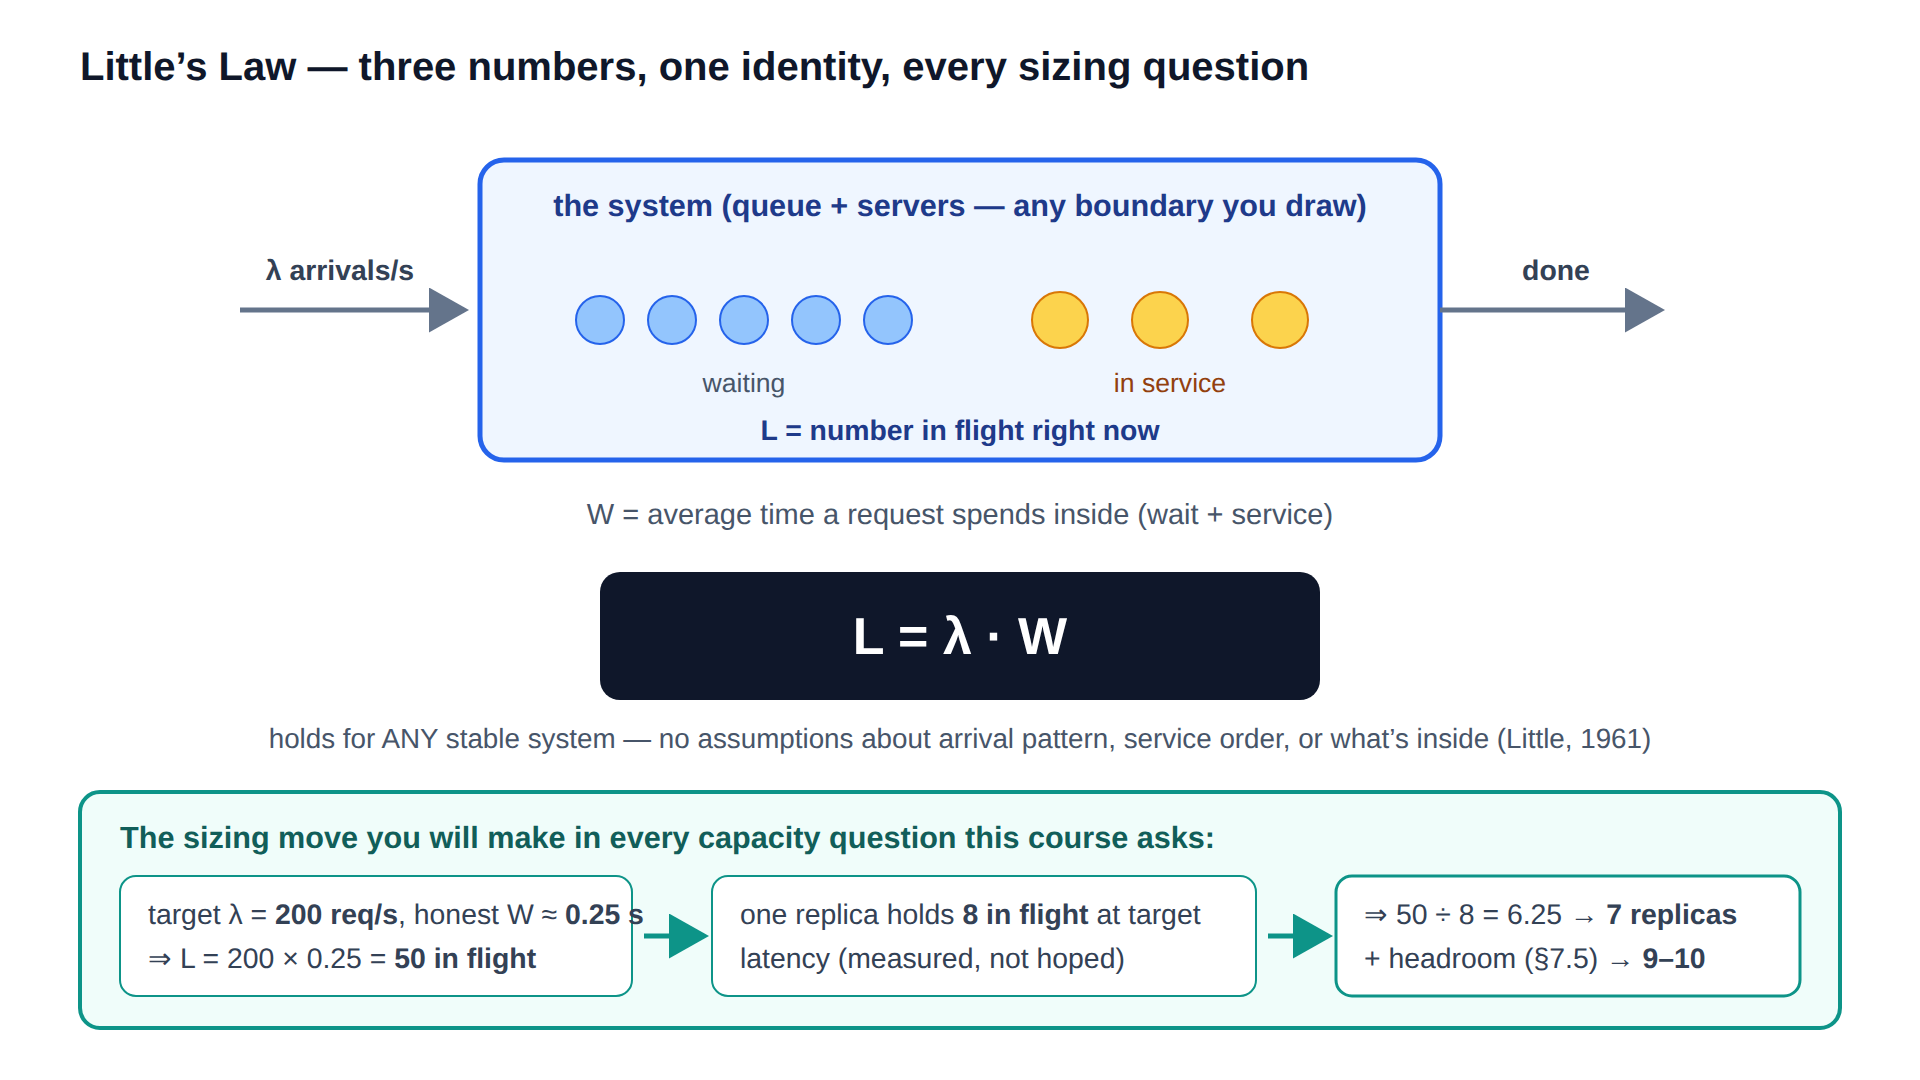
\includegraphics{figures/fig7-6_littles.png}}\\[3pt]
  \figcaption{그림 7-6  리틀의 법칙. 어떤 경계든 세 숫자와 하나의 항등식으로 설명한다. 아래에는 제안서의 용량 절에서 수행할 규모 산정 동작을 보여 준다.}
\end{tbbfigure}

주장이 너무 좋아 보이므로 터미널 기록 7-2에서 실제 서버로 확인한다. 워커 하나가 요청마다 고정 50 ms 작업을 수행하며 서로 다른 세 동시성으로 폐쇄 루프 부하를 준다.

\begin{terminalbox}
\begin{Verbatim}[breaklines=true,breakanywhere=true,fontsize=\small,formatcom=\color{tbbtermfg},codes=\tbbcodeactive]
# server: 1 worker, exactly 50 ms per request. three runs of hey:
$ hey -z 30s -c 1  http://svc/predict | grep -E "Requests/sec|Average"
  Requests/sec:  20.0      Average: 0.0500 s    # L = 20.0 x 0.050 =  1.0
$ hey -z 30s -c 10 http://svc/predict | grep -E "Requests/sec|Average"
  Requests/sec:  20.0      Average: 0.4999 s    # L = 20.0 x 0.500 = 10.0
$ hey -z 30s -c 40 http://svc/predict | grep -E "Requests/sec|Average"
  Requests/sec:  20.0      Average: 1.9998 s    # L = 20.0 x 2.000 = 40.0
# throughput is PINNED at 1/0.050 = 20/s no matter the concurrency;
# raising c only chose how much waiting existed. L = λW, every time.
\end{Verbatim}
\end{terminalbox}
\figcaption{터미널 기록 7-2  실제로 검증한 리틀의 법칙. 서버 하나, 요청당 50 ms라는 사실 하나, 세 가지 동시성에서 항등식이 소수 셋째 자리까지 성립한다. 처리량 상한(1 ÷ 서비스 시간)은 제1장 사례 A의 계산에 진짜 이름을 붙인 것이다.}

곧바로 세 가지 실용적인 용도가 나온다. 가장 중요한 아래의 \textbf{규모 산정}에서는 목표 λ와 정직한 W가 주어졌을 때 L = λW로 처리 중 요청 수를 구하고, 레플리카 하나가 처리 중으로 유지할 수 있는 수로 나눠 플릿을 정한다. \textbf{대시보드 타당성 검사}에서는 지표가 평균 400 ms에서 300 req/s라고 하면 처리 중 요청이 약 120개여야 한다. 처리 중 요청 게이지(gauge)가 15라면 세 숫자 가운데 하나가 거짓말하며, 보통 잘못된 위치에서 측정한 지연 시간이다(§7.3). \textbf{숨은 대기열 찾기}에서는 클라이언트에서 측정한 W가 서버 쪽 W보다 크면 그 차이에 리틀의 법칙을 적용해 LB, 커널 수락 대기열, GPU 배처(batcher) 가운데 \textit{보이지 않는 대기열의 위치를 좁힌다.} 제3장의 디버깅 감각이 이제 정량화되었다.

\subsection*{하키 스틱: 시스템이 90\%에서 죽는 이유}

리틀의 법칙은 \textit{현재 상태}를 세고 두 번째 결과는 운을 시험할수록 \textit{무슨 일이 일어날지} 예측한다. 레플리카 하나를 무작위 푸아송(Poisson) 도착과 지수 분포 서비스 시간을 가진 교과서적인 \textbf{M/M/1} 대기열로 모델링하고 사용률을 \textbf{ρ = λ ÷ 용량}으로 정의하자. 시스템 평균 시간은 \textbf{W = S ÷ (1 − ρ)}이며 S는 순수 서비스 시간이다. 분모를 읽어 보자. ρ = 0.5에서 W = 2S로 대기 시간이 이미 작업 시간과 같다. ρ = 0.8이면 5S, 0.9면 10S, 0.95면 20S다(그림 7-5). 곡선의 날이 SLO를 향해 치솟는 하키 스틱 모양이다. 물리적 원인은 고갈이 아니라 \textbf{변동성}이다. 무작위 도착은 \textit{뭉치며}, 용량에 가까워지면 이 뭉침을 흡수할 여유가 없다. 그래서 평균 수요가 평균 공급보다 낮아도 대기열이 생긴다. 실제 서빙 시스템에는 GPU 배치 처리, 여러 워커, 지수 분포가 아닌 서비스 시간이 있어 M/M/1보다 복잡하지만 형태는 모든 복잡성을 견디며 숫자만 달라진다.

\begin{tbbfigure}
  \adjustbox{max width=0.94\linewidth,max totalheight=0.46\textheight}{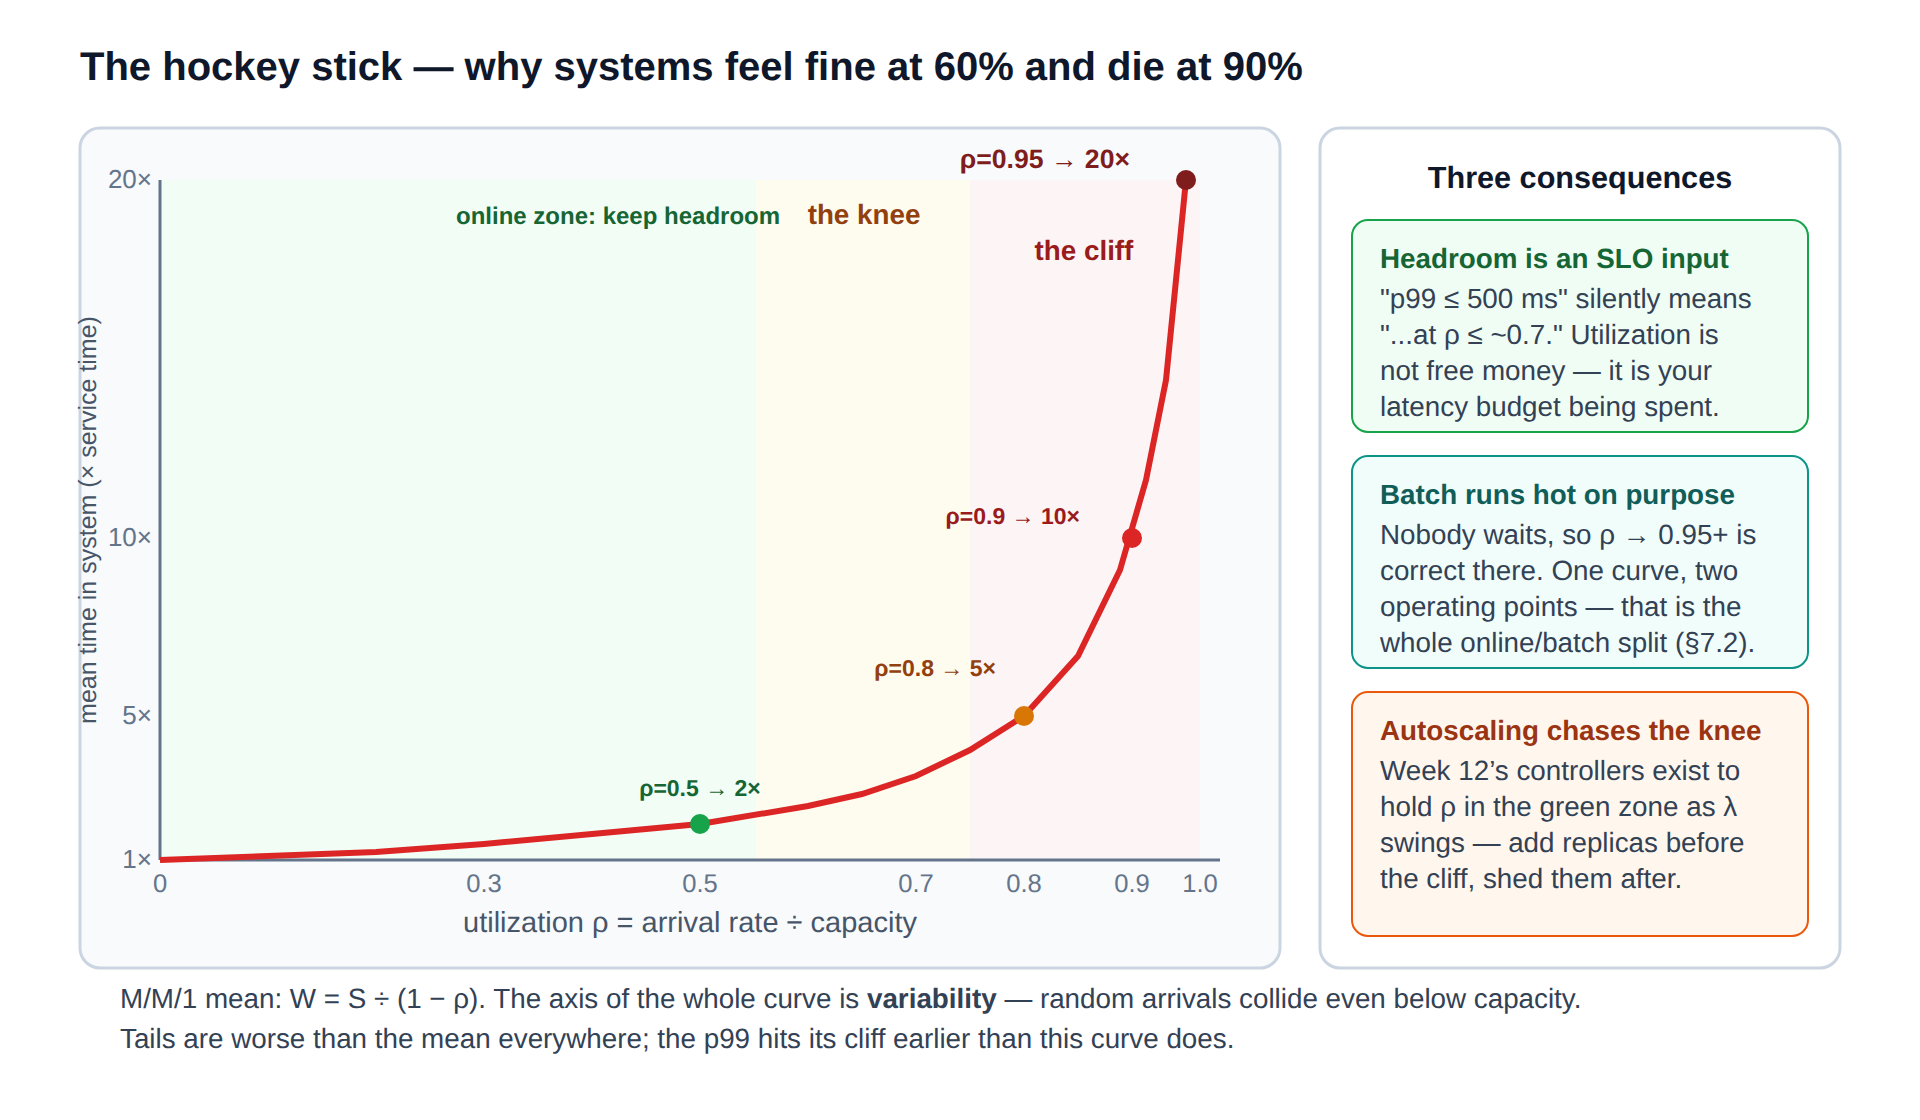
\includegraphics{figures/fig7-5_hockey.png}}\\[3pt]
  \figcaption{그림 7-5  하키 스틱 W = S ÷ (1 − ρ)와 세 가지 운영 교훈. 여유분은 SLO 입력이고, 배치는 의도적으로 뜨겁게 실행하며, 오토스케일링은 굴곡점을 따라가기 위해 존재한다.}
\end{tbbfigure}

\begin{terminalbox}
\begin{Verbatim}[breaklines=true,breakanywhere=true,fontsize=\small,formatcom=\color{tbbtermfg},codes=\tbbcodeactive]
# same 20/s-capacity server. open-loop sweeps (wrk2), 3 min per point:
  rate      rho     p50       p99
  10.0/s    0.50     69 ms    460 ms
  16.0/s    0.80    173 ms    1.2 s
  18.0/s    0.90    347 ms    2.3 s
  19.0/s    0.95    693 ms    4.6 s     # +5% load -> +100% latency
  19.8/s    0.99    3.5 s      23 s     # queue now barely drains at all
# nothing "broke," no error was logged. arithmetic happened.
# and note the tail: p99 hits YOUR SLO long before p50 looks sick.
\end{Verbatim}
\end{terminalbox}
\figcaption{터미널 기록 7-3  측정한 하키 스틱. 모든 행이 M/M/1의 예측(p50 ≈ 0.69·W, p99 ≈ 4.6·W)과 맞는다. 마지막 주석이 운영상 의미를 알려 준다. 중앙값이 아직 정상으로 보일 때 꼬리는 SLO를 위반한다.}

세 가지 결과를 기억하자(그림 7-5 오른쪽). \textbf{여유분은 SLO 입력}이다. "p99 ≤ 500 ms" 같은 약속에는 "ρ ≤ 약 0.7에서"라는 조건이 조용히 따라붙는다. 사용률은 공짜 돈이 아니라 쓰고 있는 지연 시간 예산이다. 온라인 경로에서 95\% 사용률을 좇는 플릿은 p99를 미리 써 버릴 뿐이다. \textbf{배치는 의도적으로 뜨겁게 실행}한다. 기다리는 사람이 없으면 ρ → 0.95가 \textit{옳다.} 같은 곡선의 서로 다른 두 운영 지점이며 이 구분이 §7.2의 전체 경제 논리다. \textbf{오토스케일링은 굴곡점을 따라간다.} 12주 차 컨트롤러는 λ가 움직일 때 ρ를 초록 구간에 유지하며 절벽 전에 레플리카를 추가하고 뒤에는 제거한다. 하키 스틱 때문에 HPA에 목표 사용률 필드가 있다.

\subsection*{정직한 플릿 규모 산정과 강의계획서를 가르치는 청구서}

이제 이미 가진 요소로 제안서 용량 절을 조립하자. \textbf{1단계 — 레플리카 하나를 정직하게 측정한다.} 게이트웨이를 통과하는 개방 루프 부하(§7.3)에서 SLO 지연 시간 목표가 깨질 때까지 도착률을 훑는다. L4 레플리카 하나의 양자화한 3B 모델이 \textbf{p99 = 460 ms에서 28 req/s}를 지속한다고 하자. 500 ms 약속 안에 넉넉히 들어오며 34 req/s로 밀자 꼬리가 무너졌다. 28/약 40의 포화 용량 ≈ ρ 0.7이므로 하키 스틱이 작동한 것이다. \textbf{2단계 — 리틀의 법칙으로 교차 확인한다.} 목표 200 req/s에서 정직한 평균 W ≈ 0.16 s라면 플릿 전체 L = 200 × 0.16 = \textbf{처리 중 요청 32개}다. 레플리카 8개에 각각 약 4개로 측정한 배처 깊이와 맞는다. 9주 차 실습에서 프레임워크의 처리 중 요청 게이지가 크게 다르면 보고 있지 않은 곳에 대기열이 있다. \textbf{3단계 — 나누고 올림한다.} 200 ÷ 28 = 7.1 → 피크에 \textbf{레플리카 8개}다. 포화가 아니라 SLO \textit{지점에서} 측정했으므로 여유분은 이미 28 안에 들어 있다.

\textbf{4단계 — 비용을 계산한다.} 제2장의 플릿 표를 사용하면 8 × L4(시간당 약 \$0.80) × 744 h = \textbf{월 \$4,762}다. 제안서 상한은 \$900다. 잠시 이 숫자를 바라보자. \textit{지금 종이 위에서 무료로} 발견하는 것이 이 장의 가장 가치 있는 제출물이다. 사례 1-B의 팀은 프로덕션에서 월말에 달러로 자기 숫자를 발견했다. 간격은 판결이 아니라 \textbf{강의계획서}다. 레플리카별 처리량을 두 배로 만드는 양자화(10주 차)는 플릿을 절반으로 줄인다(→ 약 \$2,381). 200 req/s 피크가 하루 약 4시간뿐이라면 일중 곡선(diurnal curve)을 따라가는 오토스케일링(12주 차)이 레플리카 시간을 다시 대략 절반으로 줄인다(→ 약 \$1,200). 더 똑똑한 배치 처리(10–11주 차)와 배치 구성 요소의 스팟 용량(12주 차)이 나머지를 메운다. \textbf{\$4,762에서 \$900로 가는 길은 거의 한 줄씩 이 강의의 후반부와 같다.} 제안서에 정직한 오늘 가격과 적용할 지렛대가 포함된 목표 가격을 모두 적자.

\begin{calloutbox}{tbbpurple}{tbbpurplefill}
{\normalsize\bfseries\color{tbbpurple}생각해 보기}\par\vspace{3pt}
\begin{tbbitemize}
  \item 이 절의 도구로 사례 1-A를 다시 계산하자. 서비스 시간 0.31 s, 레플리카 하나, 동시 사용자 100명일 때 리틀의 법칙에서 λ\_max, ρ, W는 얼마인가? 이제 게이트웨이의 30 s 타임아웃을 더하면 도착 요청 가운데 몇 \%가 504가 되는가? 제1장에서는 감으로 했지만 이제 두 줄 계산으로 보여 주자.
  \item 대시보드에 λ = 120 req/s, 평균 지연 시간 250 ms, "처리 중 요청" 게이지 90이 표시된다. 리틀의 법칙으로 세 숫자 가운데 하나가 틀렸음을 증명하고 의심 순위를 정하자. §7.3에는 이에 관한 견해가 있다.
  \item 팀원이 "유휴 GPUs는 낭비"라며 온라인 플릿을 ρ = 0.9로 실행하자고 제안한다(제1장). 터미널 기록 7-3의 행을 사용해 ρ = 0.9의 비용을 밝히는 두 문장 반론과, 그 직관이 실제로 맞는 워크로드에 적용할 §7.2의 대안을 작성하자.
  \item 4단계의 오토스케일링 추정치를 다시 도출하자. 피크 200 req/s가 하루 4시간이고 나머지는 약 60 req/s다. 레플리카마다 28 req/s라면 완벽한 오토스케일러는 하루에 레플리카 시간을 얼마나 쓰며, 고정 플릿 8개는 얼마나 쓰는가? 12주 차 콜드 스타트 문제는 "완벽"에 어떤 영향을 주는가?
\end{tbbitemize}
\end{calloutbox}

\section{모델 형식과 변환 경로}

제안서에는 빈칸 하나가 남았다. \textbf{런타임은 정확히 어떤 파일을 실행하는가?} 제6장은 객체 스토어에 버전과 다이제스트 주소가 있는 접두사를 만들고, 시작할 때 병렬 범위 GET으로 가져오는 선반을 세웠다. 선반에 \textit{무엇을 놓는지}는 이번 주에 다룬다고 약속했다. 질문은 둘로 깔끔하게 나뉜다. \textbf{가중치}를 파일에 담는 방식은 보안 교훈 하나가 붙은 이미 해결된 문제이고, \textbf{연산}을 배포하는 방식은 10주 차에 다시 볼 현재 진행형 절충 관계다. 그림 7-7이 지도다.

\begin{tbbfigure}
  \adjustbox{max width=0.94\linewidth,max totalheight=0.46\textheight}{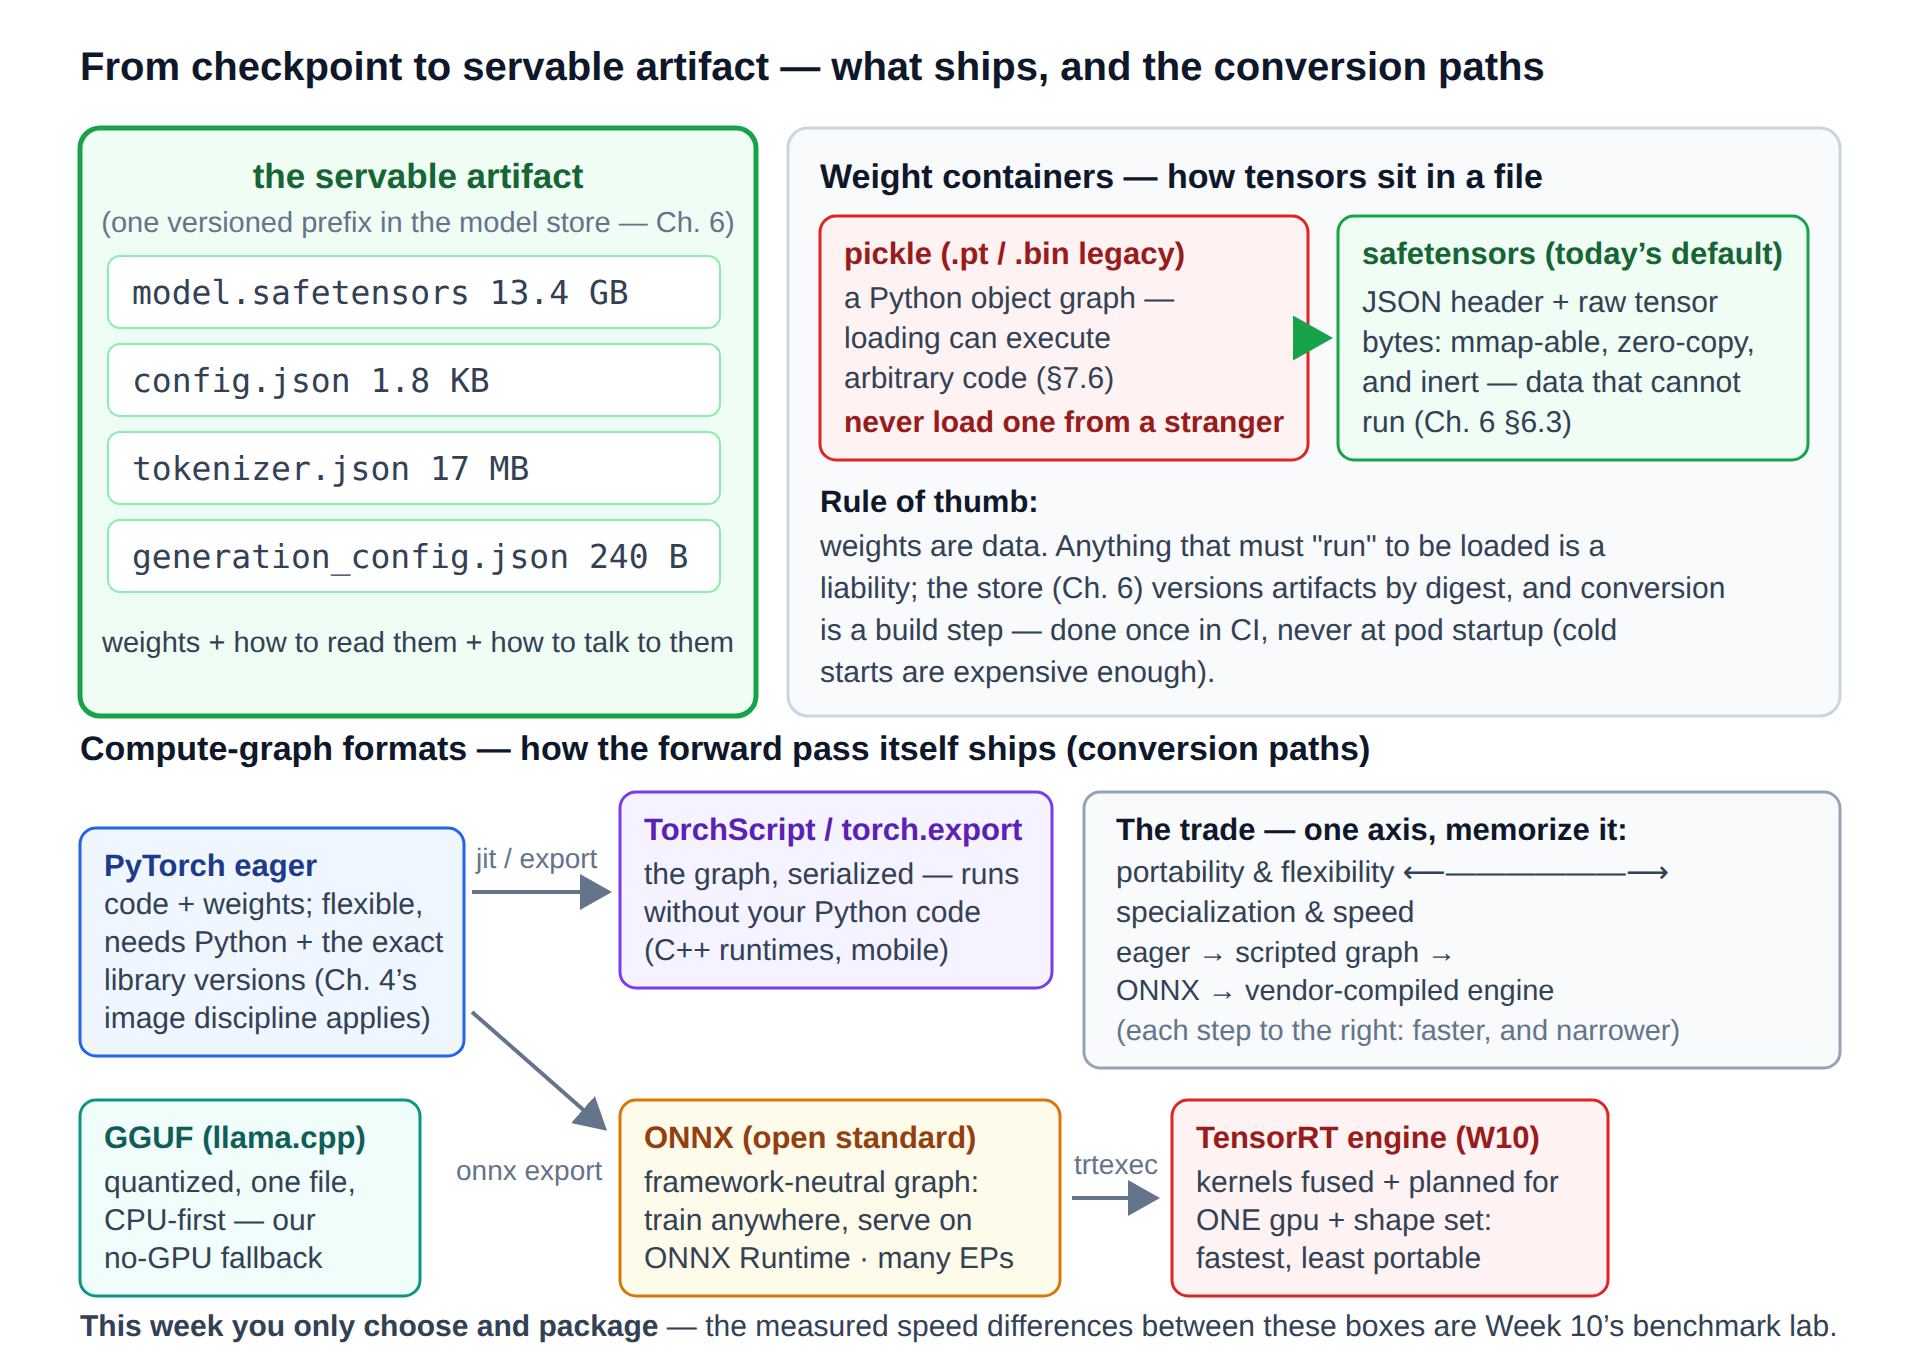
\includegraphics{figures/fig7-7_formats.png}}\\[3pt]
  \figcaption{그림 7-7  서빙 가능한 산출물과 형식. 왼쪽은 실제 배포 요소다. 위는 pickle의 위험과 safetensors를 비교한 가중치 컨테이너다. 아래는 한 축에 놓인 연산 그래프 형식으로 오른쪽일수록 빠르고 적용 범위가 좁다.}
\end{tbbfigure}

\subsection*{산출물: 가중치와 읽는 방법, 대화하는 방법}

현대 모델 디렉터리를 벗겨 내면 세 역할이 남는다(그림 7-7 왼쪽). GB 단위의 \textbf{가중치}인 \code{model.safetensors}, 계층 수·차원·활성화 함수처럼 그 GB를 \textit{배열하는 방법}을 설명하는 KB 단위 \textbf{아키텍처 구성 파일}인 \code{config.json}, 사람의 텍스트와 텐서 인덱스 사이의 계약인 \textbf{토크나이저} \code{tokenizer.json}이다. 어느 하나를 잃어도 나머지를 쓸 수 없다. 구성 파일 없는 가중치는 꼬리표 없는 이진 데이터다. 구성 파일과 가중치에 \textit{정확한} 토크나이저가 없으면 유창한 헛소리를 만든다. 모델은 "동작"하지만 토큰 4821이 더 이상 학습 때와 같은 뜻이 아니어서 단어 샐러드로 답하는 대표적이고 답답한 실패다. 세 요소가 \textbf{서빙 가능한 산출물}이며 다이제스트로 고정한 접두사 하나 아래에서 단위로 버전을 관리한다. 제4장의 태그 대 다이제스트 규율을 모델 스토어에서 다시 적용한 것이다. 제안서에는 모델, 크기, 양자화 상태, 라이선스, 산출물 배치를 명시한다.

\subsection*{Pickle 문제: 현실이 된 경고}

제6장은 safetensors가 "실행할 수 없는 데이터"라는 사양 항목으로 이를 설명했고 이번 주에 \textit{강하게} 반복하겠다고 약속했다. 이제 그 의미를 느껴 보자. PyTorch의 고전 체크포인트 형식인 \code{.pt}/\code{.bin}은 직렬화한 Python \textit{객체 그래프}인 \textbf{pickle}이다. 역직렬화기는 파일이 지정한 함수를 호출해 기꺼이 객체를 재구성한다. pickle의 버그가 아니라 계약이며, \textbf{체크포인트를 로딩하면 파일 제작자가 고른 코드가 실행될 수 있음}을 뜻한다.

\begin{terminalbox}
\begin{Verbatim}[breaklines=true,breakanywhere=true,fontsize=\small,formatcom=\color{tbbtermfg},codes=\tbbcodeactive]
$ python - <<'EOF'
import pickle
class Innocent:                    # what a "checkpoint" can smuggle
    def __reduce__(self):          # pickle: "to rebuild me, call this"
        return (print, ("hello from INSIDE your checkpoint load",))
blob = pickle.dumps(Innocent())
pickle.loads(blob)                 # merely LOADING the file...
EOF
hello from INSIDE your checkpoint load
# loads() called a function the file chose. print() today;
# os.system() in a malicious "fine-tune" you downloaded tomorrow.
$ python -c "from safetensors.torch import load_file as l; l('m.safetensors')"
# JSON header parsed, tensors mmap'd. nothing executes, ever. (Ch. 6)
\end{Verbatim}
\end{terminalbox}
\figcaption{터미널 기록 7-4  무해하게 시연한 pickle 문제. pickle을 역직렬화하면 파일이 지정한 임의의 함수를 호출할 수 있다. 그래서 "체크포인트를 다운로드했다"는 말은 코드 실행 사건을 뜻하며 생태계가 safetensors로 옮겨 갔다.}

따라오는 운영 규칙은 짧다. 어디서나 \textbf{safetensors}를 우선한다. 제6장의 mmap과 무복사 로딩을 사용하고 역직렬화(deserialization) 비용이 없어 \textit{더 빠르기도} 하다. 기존 pickle을 피할 수 없으면 \code{torch.load(..., weights\_only=True)}로 로딩한다. 최신 PyTorch가 바로 이 터미널 기록 때문에 이를 기본값으로 사용한다. 예외가 생기면 우회할 불편이 아니라 위험 신호로 본다. 조직 차원에서는 모델 파일을 \textit{인터넷에서 온 입력}으로 취급한다. 무작위 Docker 이미지(제4장)에 주는 만큼만 신뢰한다. 즉 출처와 다이제스트가 없으면 사용하지 않는다. 제6장의 보안 연습문제인 "공격자가 악성 pickle로 서빙 파드 안에서 코드 실행에 성공했다"는 이 절을 전제로 했다. 이제 첫 줄을 직접 쓸 수 있다.

\subsection*{그래프 형식: 하나의 축, 네 정거장, 변환 시점 규칙}

가중치는 비활성 데이터이므로 무언가가 여전히 \textit{계산}해야 한다. 선택지는 하나의 축에 놓인다(그림 7-7 아래). 오른쪽으로 갈수록 이식성과 유연성을 속도와 특수성에 맞바꾼다. \textbf{즉시 실행(eager execution) PyTorch}는 가중치 옆에 Python 코드를 배포한다. 가장 유연하지만 환경과도 가장 깊이 얽힌다. 정확한 라이브러리 버전이 필요해 제4장의 "내 컴퓨터에서는 된다"는 질병이 생기며 이미 갖춘 이미지 규율만 이를 막는다. \textbf{TorchScript / `torch.export`}는 그래프 자체를 직렬화해 C++ 런타임이 Python 없이 실행하게 한다. \textbf{ONNX}는 프레임워크 중립 교환 형식이다. \code{torch.onnx.export}가 표준 그래프를 만들고 \textbf{ONNX Runtime}이 CPU, CUDA, TensorRT 등의 교체 가능한 \textit{실행 제공자}로 실행한다. 어디서나 학습하고 어디서나 서빙하는 대신 연산자 지원 범위 가장자리에서 비용을 낸다. 사용자 정의 연산과 특이한 동적 형상은 잘 이동하지 못한다. 대표적으로 TensorRT인 \textbf{컴파일 엔진}은 그래프를 GPU 모델 하나와 형상 범위 하나에 맞게 \textit{계획}한다. 커널을 융합하고 정밀도를 선택하며 메모리를 미리 배치한다. 가장 빠르지만 A10G용으로 만든 엔진이 다른 곳에서는 실행되지 않을 만큼 좁다. 이 모든 것과 나란히 llama.cpp의 양자화 단일 파일 형식인 \textbf{GGUF}가 있다. 이 강의의 GPU 없는 대체 경로로 실용적으로 중요하다. 축을 따라 측정한 속도 차이는 10주 차 벤치마크 실습에서 다루며 이번 주에는 \textit{선택하고 패키징}만 한다.

두 규칙이 선택을 운영 가능하게 만든다. \textbf{변환은 빌드 단계이며 절대 시작 단계가 아니다.} 내보내기와 검증은 CI에서 한 번 실행해 다이제스트로 고정한 새 산출물을 만든다. 파드 시작은 이미 콜드 스타트의 핵심 경로이고 제6장에서 비용을 계산했다. 확장 사건마다 변환을 N번 하면 미묘하게 서로 다른 모델 N개를 만들 기회도 N번 생긴다. 또한 \textbf{변환한 모델은 동등성을 증명해야 한다.} 산출물에 버전을 부여하기 \textit{전에} 고정 입력 모음을 원본과 변환한 모델에 실행해 허용 오차 안에서 출력을 비교한다. 그래프 변환은 부동소수점 계산 순서를 합법적으로 바꾸므로 비트 단위 동일성은 잘못된 검사다. 하지만 "1e-3 안에서 가깝고 1순위가 같음"을 확인하는 다섯 줄 스크립트는 실제로 조용한 수치 오류를 찾아냈다. 동등성 검사가 없는 변환은 실제로 한 번도 시험하지 않은 모델이다.

\begin{calloutbox}{tbbpurple}{tbbpurplefill}
{\normalsize\bfseries\color{tbbpurple}생각해 보기}\par\vspace{3pt}
\begin{tbbitemize}
  \item 팀원 제안서에 "유연성을 극대화하기 위해 파드 시작 때 TensorRT로 변환한다"고 적혀 있다. 이 절을 바탕으로 콜드 스타트, 산출물 정체성, 동등성 검사라는 세 부분으로 비판하고 CI 형태의 대안을 제시하자.
  \item 토크나이저를 서빙 이미지에 구워 넣지 않고 버전이 있는 산출물 \textit{안에} 두어야 하는 이유는 무엇인가? 모델 v7이 v6의 토크나이저와 배포될 때 생기는 실패를 구성하자. 서비스는 무엇을 반환하고 §7.4의 SLI 가운데 어떤 것이 이를 알아채는가? 알아채는 것이 있는지도 생각하자.
  \item 프로젝트에서 즉시 실행 방식 / TorchScript / ONNX / TensorRT / GGUF의 순위를 매기자. 제안서에 어느 형식을 배포하고 10주 차에는 무엇을 실험할 것인가? 선택을 결정한 제약 조건인 팀 역량, 하드웨어, 모델 아키텍처를 말하자.
\end{tbbitemize}
\end{calloutbox}

\section{실습: 프로젝트 제안서 — 한 페이지와 다섯 숫자}

이번 주 제출물은 팀 프로젝트 제안서다. 사례 7-A의 팀이 수요일 회의를 하지 않아도 되게 해 줄 \textbf{한 페이지}다. 이 장의 각 절이 빈칸 하나씩을 채웠으며, 실습에서는 용량 계산의 기준이 될 정직한 측정값 하나와 함께 조립한다. 채점 기준은 상자 7-2의 문장을 확장한 것이다.

\subsection*{제안서의 다섯 절}

\begin{tbbitemize}
  \item \textbf{1 · 산출물(§7.6).} 모델, 매개변수 수, 양자화 상태, 라이선스, 정확한 산출물 배치(가중치 형식, 토크나이저, 구성 파일), 스토리지 접두사를 적는다. 모델이 pickle로 왔다면 CI에서 동등성 검사를 거쳐 safetensors 산출물이 되는 방법을 설명한다.
  \item \textbf{2 · 방식과 트래픽 분해(§7.2).} 실제로 온라인인 요청, 배치로 실행할 작업, 응답의 스트리밍 여부를 밝히고 주 경로에 표 7-2의 다섯 질문으로 답한다.
  \item \textbf{3 · SLO 문장(§7.4).} SLI, 목표값, 평가 기간, 부하 조항, 비용 상한이라는 다섯 조항을 모두 넣는다. 15주 차 데모는 이 계약을 기준으로 평가하며 12주 차 점검에서 다시 읽는다.
  \item \textbf{4 · 용량과 비용 범위(§7.5).} SLO에서 측정한 단일 레플리카 지속 가능 도착률(개방 루프, 게이트웨이 경유 — 상자 7-1), 리틀의 법칙 교차 확인, 피크 레플리카 수, 제2장 플릿 표로 계산한 정직한 월 가격, 10–12주 차에 적용할 지렛대를 포함한 오늘 가격 → 목표 가격 간격을 적는다.
  \item \textbf{5 · 위험과 대체 경로.} 모든 팀이 밝혀야 할 대표 위험 두 가지는 GPU 할당량·가용성과 감당할 수 없는 SLO다. 전자의 대안은 더 작은 모델 또는 이 강의가 보장하는 경로인 CPU의 GGUF다. 후자의 대안은 14주 차 새벽 2시가 아니라 지금 차분하게 선택하고 방어할 §7.4의 완화안이다.
\end{tbbitemize}

\subsection*{제안서의 기준이 되는 측정}

제안서의 숫자 하나는 추정이 아니라 반드시 \textit{측정}해야 한다. 모델을 대신해 서빙할 수 있는 \textbf{어떤} 대상이든 단일 레플리카 벤치마크를 처음 실행한다. 실제 후보가 이미 실행되면 그것을 쓰고, 아니면 4주 차 FastAPI 실습 서버를 쓴다. 절차는 상자 7-1을 축소한 형태다. 게이트웨이 뒤에 배포하고, 워밍업 요청은 버리며, 3–5개 도착률에서 개방 루프 탐색을 수행하고, 각각의 오류율과 \textit{함께} p50/p95/p99를 기록한다. 초안 SLO의 지연 시간 목표를 지키는 가장 높은 도착률을 찾는다. SLO에서 레플리카당 초당 요청 수로 나타낸 이 값이 강의 나머지 기간에 계산할 모든 용량 숫자의 씨앗이다. 9주 차 프레임워크 실습에서 Locust로 올바르게 다시 측정해 도구가 숫자의 정직성을 높이는 모습을 직접 확인한다.

\begin{calloutbox}{tbbred}{tbbxFEF2F2}
{\normalsize\bfseries\color{tbbx991B1B}상자 7-3  채점자가 매년 보는 제안서 실수 여섯 가지}\par\vspace{3pt}
\begin{tbbitemize}
  \item \textbf{"평균 지연 시간 ≤ X"} — 이 장이 한 절을 들여 해체한 SLI다. 백분위수를 쓰거나 아무것도 쓰지 않는다(§7.3).
  \item \textbf{부하 조항 없음} — λ를 명시하지 않고 약속한 p99는 아무것도 약속하지 않는다. 첫 버스트에서 하키 스틱이 먹어 치운다(§7.5).
  \item \textbf{정확도를 SLO로 사용} — 모델 품질은 인프라가 아니라 세상과 함께 드리프트한다. 대신 유효성·완료율 SLI를 약속하고 14주 차에 드리프트를 모니터링한다(§7.4, 표 7-3).
  \item \textbf{비용 = GPU만} — LB, NAT 외부 전송(제6장의 세금), 스토리지, 종료를 잊은 스테이징 환경에서도 계량기가 돌아간다. 사례 1-B는 계속 살아 있다.
  \item \textbf{폐쇄 루프 벤치마크 숫자} — 정중하게 기다리는 클라이언트로 측정한 용량은 개방 루프 현실보다 과장된다. 루프를 표시하지 않으면 점수를 잃는다(§7.3, 터미널 기록 7-1).
  \item \textbf{시작 때 변환} — 콜드 스타트 경로는 신성하다. 변환은 CI에서 동등성 검사와 함께 한 번만 실행한다(§7.6).
\end{tbbitemize}
\end{calloutbox}

\vspace{3.0pt}

제출물 체크리스트는 한 페이지 문서(다섯 절, SLO 문장의 다섯 조항), 벤치마크 표(도착률 × p50/p95/p99/오류율), 그리고 사례 1-B를 기억하기 위한 이번 주 측정 비용을 보여 주는 결제 콘솔 화면 캡처다. 보통 답은 2달러 미만이다. 습관이 핵심이다.

\begin{calloutbox}{tbbpurple}{tbbpurplefill}
{\normalsize\bfseries\color{tbbpurple}생각해 보기}\par\vspace{3pt}
\begin{tbbitemize}
  \item 다른 팀과 제안서를 바꾸고 상자 7-2 체크리스트를 기준으로 SLO 문장만 평가하자. 어느 조항이 빠졌거나 측정할 수 없는가? 매년 가장 흔히 빠지는 것은 부하 조항이다.
  \item SLO에서 측정한 단일 레플리카 도착률은 9 req/s이고 목표는 200 req/s다. L4에서 레플리카 23개, 월 약 \$13,700다. 이 장과 강의계획서의 지렛대 가운데 처음 당길 세 가지는 무엇이며 각각 무엇을 현실적으로 얻는가? 올바른 첫 답이 있으며 "GPU를 더 산다"는 아니다.
  \item 새벽 2시 버전을 작성하자. 14주 차이고 SLO가 위반되었으며 데모는 6일 뒤다. 제안서의 어느 조항을 적용하는가? 이 장이 7주 차에 무엇을 미리 적게 했기에 새벽 2시 결정이 논쟁이 아니라 읽기 문제가 되는가?
\end{tbbitemize}
\end{calloutbox}

\namedsection{요약}{열두 가지로 정리한 이 장}

\qitem{1}{\textbf{합의한 숫자가 없는 서비스에서는 정상과 고장을 구별할 수 없다.} 사례 7-A의 논쟁에는 틀린 사람이 없었고 문장 하나만 빠져 있었다. 해결책은 SLI → SLO → SLA 사다리이며 그 문장을 작성하는 것이 이번 주 제출물이다.}

\qitem{2}{\textbf{지연 시간은 분포이고 평균은 아무도 설명하지 못한다.} 사례 7-B의 평균 182 ms는 p50(92 ms)과 p90 사이에 있었지만 누구도 경험하지 않았다. 반면 매일 사용자 100명이 p99 = 2.1 s보다 느린 경험을 했다. 서빙은 백분위수로 말한다. p50은 일반적 경험, p99는 매일 만나는 집단, p99.9는 CEO의 실시간 데모다.}

\qitem{3}{\textbf{속도가 곧 매출이다.} Amazon의 +100 ms → 매출 −1\%, Google의 +400 ms → 검색 −0.59\%와 지연 제거 뒤에도 지속된 효과, Mayer의 +500 ms → 트래픽 −20\% 같은 고전적 실험은 20년 뒤에도 방향이 반복된다. 지연 시간은 비용 항목이다.}

\qitem{4}{\textbf{"누가 무엇을 기다리는가?"라는 방식 질문이 전체 시스템의 형태를 결정한다.} 온라인은 꼬리를, 배치는 비용을(뜨겁게 실행, 스팟 사용, 기다리는 사람 없음), 스트리밍은 체감 속도를(첫 결과 도착 시간 + 이후 전송 속도) 관리한다. 가장 저렴한 지연 시간 최적화는 아무도 기다리지 않았음을 발견하는 것이다.}

\qitem{5}{\textbf{백분위수 문법:} 백분위수에는 평가 기간, 사용자와 가까운 측정 위치, 부하가 필요하다. 파이프라인 단계 전체에서 더할 수 없고 레플리카 전체에서 평균할 수도 없다. 백분위수가 아니라 히스토그램을 집계해야 한다. 14주 차 Prometheus가 버킷을 전송하는 이유다.}

\qitem{6}{\textbf{팬아웃에서는 꼬리가 증폭된다}(Dean \& Barroso). 호출마다 1\% 느림 × 100곳 팬아웃이면 사용자 요청의 63\%가 느린 호출을 만난다. 그래서 팬아웃을 얕게 하고 호출별 타임아웃과 헤지 요청을 사용한다. 비용을 써서 꼬리를 되산다.}

\qitem{7}{\textbf{부하 테스트는 협조적 누락으로 거짓말한다.} 폐쇄 루프 시험기는 서버가 멈춘 바로 그때 전송을 멈춘다(터미널 기록 7-1: p99 = 13 ms 대 개방 루프의 진실 1.14 s). SLO 질문에는 고정 도착률의 개방 루프 부하와 상자 7-1의 위생 규칙이 필요하다.}

\qitem{8}{\textbf{SLO에는 다섯 조항}인 SLI, 목표값, 평가 기간, 부하 조항, 비용 상한이 있고 여집합은 오류 예산(99.9\%/30일 ≈ 43분)이다. 성적표가 아니라 출시·동결 정책이다. 100\%는 잘못된 목표다. 9 하나마다 비용이 약 10배 늘지만 사용자의 잡음 바닥으로 사라진다.}

\qitem{9}{\textbf{리틀의 법칙(L = λ·W)은 안정적인 모든 경계에 성립}하는 서빙의 보존 법칙이다. 플릿 규모 산정, 대시보드 타당성 검사(λ·W = 처리 중 요청 수여야 함), 숨은 대기열 위치 찾기에 사용한다. 제1장 사례 A의 계산을 정식화한 것이다.}

\qitem{10}{\textbf{하키 스틱(W = S ÷ (1−ρ)) 때문에 시스템이 90\%에서 죽는다.} ρ = 0.5에서 이미 대기 시간과 작업 시간이 같고, ρ = 0.9에서 0.95로 가면 다시 두 배가 된다. 여유분은 SLO 입력이고 배치는 의도적으로 뜨겁게 실행하며 오토스케일링은 굴곡점을 따라가기 위해 존재한다(12주 차).}

\qitem{11}{\textbf{플릿 규모 산정은 측정 + 나눗셈이다.} SLO에서 단일 레플리카의 도착률(개방 루프, 게이트웨이 위치) → 레플리카 수 = ceil(목표 λ ÷ 레플리카당 도착률) → 플릿 표로 비용을 계산한다. 예제의 첫 청구서인 \$4,762 대 \$900 상한은 실패가 아니다. 간격이 10–12주 차 강의계획서다.}

\qitem{12}{\textbf{서빙 가능한 산출물 = 가중치 + 구성 파일 + 토크나이저이며 다이제스트로 고정한 단위 하나로 버전을 관리한다.} Pickle 체크포인트는 로딩 때 코드를 실행할 수 있으므로(터미널 기록 7-4) safetensors를 우선하고, 아니면 \code{weights\_only=True}를 사용한다. 그래프 형식은 이식성을 속도와 맞바꾼다(즉시 실행 → TorchScript → ONNX → TensorRT, CPU 대안은 GGUF). 변환은 동등성 검사를 포함한 CI 빌드 단계이며 절대 파드 시작 단계가 아니다.}

\namedsection{연습문제}{}

\subsection*{A. 객관식}

\qitem{1}{파이프라인이 매일 밤 전체 문서 말뭉치를 다시 임베딩하며 결과는 06:00까지 준비되어야 한다. 개별 임베딩을 기다리는 사용자는 없다. 알맞은 방식과 사용률 자세는?}

\begin{tbboptions}
  \item ① 온라인 — 꼬리를 위해 ρ ≤ 0.7 유지        ② 배치 — GPU를 뜨겁게 실행(ρ → 0.95), 스팟에 적합, 마감 시각 SLO
  \item ③ 스트리밍 — 첫 임베딩 도착 시간 최적화        ④ 온라인 — 06:00 마감 시각이 지연 시간 목표이기 때문
\end{tbboptions}

\qitem{2}{사례 7-B(요청 10,000건, p50 = 92 ms, 평균 = 182 ms, p99 = 2,140 ms)에서 옳은 설명은?}

\begin{tbboptions}
  \item ① 요청 10,000건 가운데 약 100건이 2,140 ms보다 오래 걸렸다.
  \item ② 사용자 대부분이 대략 182 ms를 경험했다.
  \item ③ p99가 평균의 10×를 넘으므로 반드시 잘못되었다.
  \item ④ 요청 절반이 182 ms보다 오래 걸렸다.
\end{tbboptions}

\qitem{3}{팬아웃한 하위 호출 10개가 각각 독립적으로 1\%만 느리고 요청은 모두를 기다린다. 느린 호출을 하나 이상 만나는 사용자 요청 비율은 대략 얼마인가?}

\begin{tbboptions}
  \item ① 0.1\%        ② 1\%        ③ \textasciitilde{}10\%        ④ 63\%
\end{tbboptions}

\qitem{4}{서버가 분마다 한 번씩 1.5 s 동안 완전히 멈춘다. 보고된 p99에 이 멈춤을 드러낼 부하 테스트 설정은?}

\begin{tbboptions}
  \item ① 폐쇄 루프, 동시 연결 64개, 2분 실행
  \item ② 더 많은 연결(256개)을 사용한 폐쇄 루프
  \item ③ 용량에 가까운 고정 도착률의 개방 루프, 여러 분 실행
  \item ④ 충분히 오래 실행하기만 하면 어떤 도구든 가능
\end{tbboptions}

\qitem{5}{§7.4의 구조에 따라 완전한 SLO는?}

\begin{tbboptions}
  \item ① "p99 ≤ 500 ms" 
  \item ② "게이트웨이에서 500 ms 안에 처리한 요청이 이동식 30일마다 99.5\% 이상이며, 최대 200 req/s 부하에서 월 \$900 이하"
  \item ③ "평균 지연 시간 ≤ 200 ms, 가용성 99.99\%를 영원히 유지"
  \item ④ "언제나 최대한 빠르게"
\end{tbboptions}

\qitem{6}{가용성 SLO가 30일 동안 99.9\%(오류 예산 약 43분)다. 9일째의 사고가 50분을 사용했다. 오류 예산 정책에 따라 어떤 일이 일어나는가?}

\begin{tbboptions}
  \item ① 아무 일도 없다. 예산은 권고 사항이다.
  \item ② 사전 합의에 따라 출시를 동결하고 이동식 평가 기간이 회복될 때까지 신뢰성 작업에 집중한다.
  \item ③ 사고에 맞게 SLO를 소급해 느슨하게 한다.
  \item ④ 사후 분석(postmortem) 뒤 오류 예산이 즉시 초기화된다.
\end{tbboptions}

\qitem{7}{서비스가 평균 시스템 시간 W = 0.3 s에서 λ = 80 req/s를 받는다. Little's Law에 따른 평균 처리 중 요청 수는?}

\begin{tbboptions}
  \item ① 24        ② 267        ③ 80        ④ 도착 분포를 모르면 결정할 수 없다.
\end{tbboptions}

\qitem{8}{온라인 플릿이 ρ = 0.9(평균 지연 시간 ≈ 서비스 시간의 10배, M/M/1)로 실행된다. 트래픽이 5\% 늘어 ρ ≈ 0.95가 되었다. 모델이 예측하는 평균 지연 시간은?}

\begin{tbboptions}
  \item ① 부하 증가와 같은 +5\%        ② 대략 두 배인 서비스 시간의 약 20배
  \item ③ ρ = 1.0까지 변화 없음        ④ +50\%
\end{tbboptions}

\subsection*{B. 단답형}

\qitem{1}{서버가 멈춘 바로 그동안 도구도 부하 생성을 멈추는 부하 테스트 병리의 이름을 말하고, 보고된 백분위수가 틀린 이유를 한 문장으로 설명하자.}

\qitem{2}{목표 부하는 120 req/s이고 레플리카 하나가 SLO 지연 시간 목표에서 25 req/s를 지속한다(개방 루프 측정). 피크에 레플리카가 몇 개 필요하며 별도의 여유 계수를 더하지 않아도 되는 이유는 무엇인가?}

\qitem{3}{기존 .pt 체크포인트를 로딩하면 공격자가 고른 코드를 실행할 수 있는 이유와 safetensors 파일은 그럴 수 없는 이유를 각각 한 문장으로 설명하자.}

\qitem{4}{가용성 SLO 99.5\%의 30일 오류 예산을 분 단위로 계산하자.}

\qitem{5}{이 강의에서 완전한 SLO 문장에 필요한 다섯 조항을 나열하자.}

\subsection*{C. 논술형}

\qitem{1}{§7.4의 메커니즘을 도입한 팀의 사고 서사로 사례 7-A를 다시 쓰자. PM의 보고, SLI·현재 소진량·§7.3의 히스토그램 증거가 있는 엔지니어 답변, 오류 예산 정책이 만드는 결정을 포함한다. 그런 다음 이 메커니즘이 제거한 조직적 논쟁과 의도적으로 보존한 엔지니어링 논쟁을 한 문단으로 밝히자.}

\qitem{2}{제안서의 용량 절을 설계하자. SLO에서 L4 레플리카마다 22 req/s를 측정했고 피크는 하루 \textasciitilde{}3시간 150 req/s, 나머지는 \textasciitilde{}40 req/s이며 L4 ≈ \$0.8/hr다. 고정 플릿 월 비용과 이상적인 오토스케일 비용을 계산하고 하나 또는 혼합안을 권고한다. 오토스케일링이 도입하는 위험(12주 차 예고)과 해결 전까지 보호해 주는 §7.4 조항을 말하자.}

\qitem{3}{문서 질의응답 제품은 매일 밤 말뭉치 임베딩을 수행하고, 요청 안에서 질의별 검색 + 재순위 결정을 하며, 답을 토큰별로 스트리밍한다. §7.2의 방식으로 분해하고 구성 요소마다 SLI와 목표값을 고른 뒤(표 7-3), §7.3의 팬아웃 논리에 따라 어느 구성 요소의 꼬리가 사용자 경험을 지배하는지 찾자.}

\qitem{4}{프로젝트 형식 계획을 옹호하자. 원본 체크포인트 형식과 위험(§7.6), 9주 차에 배포할 서빙 형식, 10주 차에 시도할 변환, 각 변환을 실행할 위치(CI 대 시작 단계와 근거), 승격을 제어할 동등성 검사를 포함한다. GGUF/CPU 대체 경로와 그에 따라 강제될 SLO 변경도 밝힌다.}

\namedsection{정답과 해설}{}

\subsection*{A. 객관식}

\qitem{1}{\textbf{②} 항목 하나를 기다리는 사람이 없으므로 배치다. 뜨겁게 실행하고 중단(스팟)을 감수하며 마감 시각을 최신성 SLO("아침의 99\% 이상에서 06:00까지 출력 완료")로 약속한다. ④는 작업 마감 시각과 요청별 지연 시간을 혼동했다. (§7.2)}

\qitem{2}{\textbf{①} p99 = 2,140 ms는 10,000의 1\%인 약 100건의 요청이 더 느렸다는 뜻이다. ②는 p50과 p90 사이에서 아무도 설명하지 못한 평균의 오류다. ④는 평균과 중앙값을 혼동했고, ③은 희망 사항이다. 꼬리가 두꺼우면 p99가 평균의 10–20배가 되는 일이 흔하다. (§7.3)}

\qitem{3}{\textbf{③} 1 − 0.99¹⁰ ≈ 9.6\%다. ④의 63\%는 본문의 100곳 팬아웃이다. 팬아웃이 10분의 1이어도 호출별 1\%가 10배 증폭된다. 꼬리는 증폭된다. (§7.3)}

\qitem{4}{\textbf{③} 개방 루프 부하만 멈춤 중에도 계속 도착하므로 실제 사용자가 만들 대기열을 측정한다(터미널 기록 7-1). 폐쇄 루프 연결을 늘리면(②) 멈춤 표본이 조금 늘지만 여전히 서버와 함께 멈춘다. 실행 시간을 늘려도(④) 누락을 고치지 못한다. 도구는 매번 멈춤 \textit{중}을 빼기 때문이다. (§7.3)}

\qitem{5}{\textbf{②} 다섯 조항이 모두 있다. SLI(게이트웨이에서 500 ms 미만인 비율), 목표값(99.5\%), 평가 기간(이동식 30일), 부하 조항(≤ 200 req/s), 비용 상한(\$900/월)이다. ①은 평가 기간·부하·비용이 없고, ③은 평균과 감당하기 어려운 9의 개수를 사용하며 끝나는 평가 기간이 없다. ④는 사례 7-A다. (§7.4)}

\qitem{6}{\textbf{②} 오류 예산(약 43분)을 넘겨 썼으므로 사전 합의한 정책이 발동한다. 출시를 동결하고 이동식 평가 기간이 회복될 때까지 신뢰성 작업을 한다. 결과를 사고 \textit{전에} 합의했다는 점이 이 메커니즘의 정치적 가치다. (§7.4)}

\qitem{7}{\textbf{①} L = λ·W = 80 × 0.3 = 24다. ④는 법칙의 일반성이 제거하는 함정이다. 리틀의 법칙에는 분포 가정이 전혀 필요하지 않으므로 대시보드에 안전하게 사용할 수 있다. (§7.5)}

\qitem{8}{\textbf{②} W = S ÷ (1−ρ)이므로 0.9에서는 10S, 0.95에서는 20S다. 절벽 가까이에서는 부하 5\% 증가가 지연 시간을 두 배로 만든다. 이 비대칭 때문에 여유분이 SLO 입력이고 오토스케일러는 지연 시간만이 아니라 사용률에 반응한다. 지연 시간이 움직일 때는 이미 절벽 위다. (§7.5)}

\subsection*{B. 단답형}

\qitem{1}{\textbf{협조적 누락.} 도구의 처리 중 요청이 서버와 함께 멈추므로 사용자가 대기열을 만들 바로 그 기간에는 표본이 거의 기록되지 않는다. 최악의 경험을 제외한 생존 모집단으로 백분위수를 계산한다. (§7.3)}

\qitem{2}{ceil(120 ÷ 25) = \textbf{레플리카 5개}다. 25 req/s는 포화가 아니라 SLO 지연 시간 목표 \textit{지점에서} 측정했다. 하키 스틱 절벽까지의 거리인 여유분이 이미 숫자 안에 있다. 계수를 하나 더 곱히면 이중 계산이다. (§7.5)}

\qitem{3}{.pt는 pickle이다. 역직렬화는 파일이 지정한 함수(\code{\_\_reduce\_\_})를 호출해 Python 객체 그래프를 재구성하므로 로딩 때 제작자가 고른 코드가 실행된다. safetensors는 JSON 헤더와 원시 텐서 바이트로 된 mmap 가능한 순수 데이터라 악용할 실행 단계가 없다. (§7.6)}

\qitem{4}{30일의 0.5\%는 43,200분 × 0.005 = \textbf{216분}(3.6시간)이다. 학생 SLO로 99.5\%는 방어할 수 있지만 99.99\%(약 4.3분)는 그렇지 않은 이유 가운데 하나다. (§7.4)}

\qitem{5}{\textbf{SLI · 목표값 · 평가 기간 · 부하 조항 · 비용 상한.} ("게이트웨이에서 500 ms 미만인 요청의 비율" · "≥ 99.5\%" · "이동식 30일" · "최대 200 req/s" · "월 \$900 이하") (§7.4)}

\subsection*{C. 논술형(채점 기준)}

\qitem{1}{엔지니어 답변에 평균이 아닌 \textit{정의된 SLI}, 현재 평가 기간의 소진량("43분 가운데 28분 사용" 또는 지연 시간 SLI 대응값), CEO 표본의 위치를 보여 주는 히스토그램 증거(p99.9)가 있는지 확인한다. 오류 예산에서 기계적으로 따라오는 동결 또는 출시 결정과 마지막 구분도 있어야 한다. 메커니즘은 \textit{"느린가?"}라는 논쟁을 산술로 바꿔 제거하면서, 제안 단계에서 제대로 다퉈야 할 제품 결정인 \textit{"무엇을 약속해야 하는가?"}는 보존했다. PM의 불만 접수 채널 자체가 치우친 꼬리 표본임을 알아채면 보너스다(§7.1). (§§7.1, 7.3, 7.4)}

\qitem{2}{고정 플릿은 ceil(150/22) = 레플리카 7개 × 월 \$595 ≈ \textbf{\$4,166}이다. 이상적인 오토스케일은 레플리카 7개 × 3시간 + ceil(40/22) = 레플리카 2개 × 21시간 ≈ 하루 63 레플리카 시간 대 168 → 약 37\%, 즉 \textbf{월 \$1,560}다. 좋은 답은 2개 아래로 내려가지 않는 하한 있는 오토스케일링을 권하고 콜드 스타트 위험을 말한다. 새 레플리카가 이미지를 가져오고 가중치를 로딩하는 데 몇 분이 걸려 버스트가 스케일러를 앞지른다(12주 차, 제6장에서 가져오기 비용 계산). 확장 문제를 해결하기 전에는 명시한 λ까지만 약속이 성립하도록 SLO의 부하 조항을 계약적 보호 장치로 적용한다. (§7.5)}

\qitem{3}{분해는 말뭉치 임베딩 = 배치(최신성 SLO, 뜨겁게 실행, 스팟에 적합), 검색 + 재순위 결정 = 온라인(게이트웨이의 꼬리 SLI, 팬아웃 구성원), 토큰 생성 = 스트리밍(첫 토큰 도착 시간 + 완료율 SLI)이다. 사용자의 체감 지연 시간은 스트림 앞의 \textit{온라인 팬아웃}이 지배한다. 검색 + 재순위 결정이 첫 토큰의 순차 사전 조건이므로 p99가 첫 토큰 도착 시간을 제어한다. 백분위수를 더할 수는 없지만 가장 느린 사전 조건이 지배한다. 그 뒤 스트림이 나머지를 숨긴다. 이 관찰을 스트리밍 전 팬아웃을 얕게 하고 타임아웃을 엄격하게 설정하는 것과 연결해야 한다. (§§7.2, 7.3)}

\qitem{4}{원본의 위험을 솔직히 밝힌다. pickle이면 터미널 기록 7-4, 허브의 safetensors면 다이제스트 고정을 언급한다. 9주 차 배포는 유연성을 위한 즉시 실행 방식 또는 TorchScript, CPU 중심이면 GGUF가 방어 가능하다. 10주 차 실험은 ONNX Runtime 또는 TensorRT이며 이식성 대 속도의 절충 관계를 밝힌다. CI에서 다이제스트로 고정한 출력으로 변환하고 콜드 스타트 논거에 따라 시작 경로에는 변환이 없음을 명시한다. 동등성 관문은 고정 입력 모음, 허용 오차 + 1순위 일치다. GGUF 대체 경로의 SLO 결과도 정성적으로 수량화한다. CPU 추론이라면 지연 시간 목표를 느슨하게 하거나 부하 조항을 낮추는 정직한 §7.4 재협상을 미리 선택한다. (§7.6)}

\namedsection{더 읽을거리}{}

\textbf{[이번 주]} 표시가 붙은 항목은 이번 주 필독 또는 강력 권장 자료다. \textbf{[N주 차]} 표시는 해당 주에 도움이 될 자료를 뜻한다.

\begin{tbbitemize}
  \item \textbf{[이번 주] Google SRE Book (2016), Chapter 4, "Service Level Objectives"} — 온라인에서 무료로 읽을 수 있으며 이 장이 그대로 받아들인 SLI/SLO/SLA 사다리와 오류 예산의 정석 자료다. 제안서 SLO 문장을 쓰기 전에 읽자. Appendix "Embracing Risk"(Ch. 3)와 잘 어울린다.
  \item \textbf{[이번 주] J. Dean \& L. A. Barroso, "The Tail at Scale," CACM 2013} — 팬아웃 계산, 꼬리를 평균으로 없앨 수 없는 이유, 헤지·연결 요청 완화책을 다룬 8페이지 논문이다. 해당 10년간 가장 많이 인용된 서빙 시스템 논문이자 §7.3의 63\%가 나온 곳이다.
  \item \textbf{[이번 주, 재미] Gil Tene, "How NOT to Measure Latency" (talk, various years; HdrHistogram docs)} — 쇼맨의 즐거움으로 진행하는 협조적 누락 강연이다. 보고 나면 폐쇄 루프 p99를 다시는 믿지 못한다. wrk2와 HdrHistogram이 가져갈 도구다.
  \item \textbf{속도가 곧 매출이라는 고전 자료} — G. Linden의 2006 talk notes("Make Data Useful", +100 ms Amazon experiment), J. Brutlag의 "Speed Matters for Google Web Search"(2009), M. Mayer의 Web 2.0 2006 talk(30-results 이야기)다. 짧고 오래되었지만 모두가 여전히 인용한다. §7.1의 한계에 따라 비판적으로 읽자.
  \item \textbf{J. D. C. Little, "A Proof for the Queuing Formula L = λW," Operations Research 9(3), 1961} — 놀랄 만큼 읽기 쉬운 원 논문이다. 교과서 깊이의 더 넓은 도구 모음은 L. Kleinrock의 \textit{Queueing Systems, Vol. 1}(1975)이 여전히 표준이다. 이 강의 필요를 훨씬 넘지만 M/M/1 장은 §7.5의 엄밀한 토대다.
  \item \textbf{[9주 차] Locust documentation (constant-throughput load shapes)} — 다음 주 실습 도구다. 개방 루프 도착을 표현하는 방식을 살펴보고 첫날부터 상자 7-1 체크리스트를 locustfile에 연결하자.
  \item \textbf{[10주 차] ONNX \& ONNX Runtime docs (execution providers) · TensorRT developer guide (builder, engines) · safetensors format spec} — §7.6의 상자를 구현 깊이로 다룬다. 지금 훑어보고 10주 차 실습에서 벤치마크한다.
  \item \textbf{PyTorch security note on `torch.load` and `weights\_only`} — 기존 체크포인트의 공식 마이그레이션 경로를 포함한 터미널 기록 7-4 교훈의 공식 설명이다.
\end{tbbitemize}

\vspace{5.0pt}

\begin{calloutbox}{tbbblue}{tbbbluefill}
{\normalsize\bfseries\color{tbbblue}다음 주 — 중간고사, 이어서 제9장: 모델 서빙 프레임워크}\par\vspace{3pt}
\textbf{8주 차에는 중간고사}를 치른다. 1–7주 차의 플랫폼(가상화, 컨테이너, Kubernetes, 스토리지·네트워킹)과 이 장의 서빙 어휘를 평가한다. 가장 좋은 준비는 이 책이 계속 설계해 온 방식이다. 터미널 기록을 다시 실행하고(터미널 기록 2-1부터 7-4까지 모든 어두운 상자를 재현할 수 있다), 기념품인 종료 코드 137, PID 41288, 1956 상자, 플릿 표, 삼각형, 이제 L = λW까지 따라가자. 각 기념품이 나온 장과 다시 등장한 지점을 설명할 수 있으면 준비가 된 것이다.

\textbf{제9장}에서는 모델 아래에 전문 서빙 프레임을 놓는다. Triton Inference Server, TorchServe, BentoML, Ray Serve를 살펴보고, "서빙 프레임워크"가 4주 차 FastAPI 서버에 실제로 추가하는 동적 배치 처리(dynamic batching), 모델 관리, 지표 엔드포인트, 다중 모델 라우팅, 선택 방법, 제안서 용량 숫자를 정직하게 만드는 Locust 부하 테스트를 다룬다. 이 장의 백분위수 규율을 가지고 가자. 곧 도구를 만난다.
\end{calloutbox}
